\documentclass[minf,frontabs,twoside,singlespacing,parskip]{infthesis} 

\usepackage{url}
\usepackage{graphicx}
\usepackage{subfig}
\usepackage{wrapfig}

%\usepackage{biblatex}
%\usepackage[xetex]{graphicx}
%
%\usepackage{fontspec,xunicode}
%
%\defaultfontfeatures{Mapping=tex-text,Scale=MatchLowercase}
%\setmainfont[Scale=.95]{Georgia}
%\setmonofont{Georgia}


\usepackage{amsmath}
\newcommand{\BigO}[1]{\ensuremath{\operatorname{O}\bigl(#1\bigr)}}

\usepackage{listings}
\usepackage{color}

\definecolor{dkgreen}{rgb}{0,0.6,0}
\definecolor{gray}{rgb}{0.5,0.5,0.5}
\definecolor{mauve}{rgb}{0.58,0,0.82}

\lstset{frame=tb,
  language=Python,
  aboveskip=3mm,
  belowskip=3mm,
  showstringspaces=false,
  columns=flexible,
  basicstyle={\small\ttfamily},
  numbers=left,
  numberstyle=\tiny\color{gray},
  keywordstyle=\color{blue},
  commentstyle=\color{dkgreen},
  stringstyle=\color{mauve},
  breaklines=true,
  breakatwhitespace=true
  tabsize=4
}

\begin{document}
\title{Modelling search volumes as a dynamic system responding to external events}

\author{Stefan Sabev}

\course{Master of Informatics}
\project{{\bf MInf Project (Part 1) Report}}

\date{\today}

\abstract{
It is well known that some events might spark people's interest to fly to different destinations. In particular news events or sports events can quite easily make people search for a specific destination - for example the Champions League Quarter final draw increased the number of flight searches from Glasgow to Spain 6 times.\\
For this project we have collected vast amounts of Twitter data. With this dataset and the flight search dataset provided by Skyscanner it was possible to build a model that predicts flight search demand based on what's happening on Twitter. This is a noble approach to predicting flight search volumes utilising the vastness of Social data available. \\
The potential applications of this are generic prediction of flight search volumes, predicting new events for better marketing and also anomaly detection in traffic caused by events.
}

\maketitle

%\section*{Acknowledgements}

%I would like to thank Charles Sutton for his support while supervising this project and for all the suggestions that made it possible.\\
%\\
%Another thank you goes to Ewan Nicolson for helping with the project and giving access to data storage and the Skyscanner dataset used in this project.

\tableofcontents

\pagenumbering{arabic}

\chapter{Introduction and background}

\section{Introduction}

There aren't that many flight search companies with the global outreach required to collect and aggregate massive volumes of flight search data. And there are even fewer ones that are making some or the whole of their datasets available for research. When you consider that and the fact that online travel is a niche area in itself, one starts to understand why research of this kind would have been quite hard if not impossible to do up until this date. However as some of those companies grow, they are trying to employ more sophisticated ways of predicting demand and as a result of that plan their hardware capacity better or just use that data for revenue forecasting. With the rise of social media, the next logical step would be to start exploring different ways of adding exogenous factors such as data extracted from Twitter into their models to better their prediction. 


In this project you will find the first attempt that someone has made to try using and incorporating social media to predict flight searches. As a consequence of that the effect of social media over online travel can be measured. We will try to show that using this dataset (\textasciitilde 500GB at the time of writing, 565 million tweets as time of writing) we can employ text mining and try to build a model that can predict upward and downward shifts in demand for a group of destinations - countries and cities as of the first part. With NLP we will hopefully gain better understanding on how to predict demand and therefore this could be useful not just to flight search companies, but also to airlines and airports. 


It will be impossible not to say anything about Skyscanner, since they have kindly provided the flight search data, which I am using in this project. \footnote{\textbf{Dislaimer}: I am an employee of the company and have been working there since 2011} It's an Edinburgh-based company with offices around the whole world, which is slowly, but surely positioning itself as a leader in travel search online. It is in the phase of rapid growth and it has been doubling in size and valuation for the past couple of years, which helped secure an investment from Sequioa Capital \cite{seqcap}.  

Due to the fact it processes billions of user searches on a monthly basis it is quite important to be able to predict roughly what tomorrow is going to look like, because there could be a knock-on effect on the capacity and website performance or the costs in general. This has made Skyscanner transform from a flight search company into a data-driven company. With "Big Data" comes big responsibility - you need to get the maximum value out of your data rather than just store it on disk. In order to utilise all of it they have developed and deployed a lot of in-house algorithms for anomaly detection and force sating all of their KPIs (Key Performance Indicator). However there are still some things that you can't predict from just looking at past data and learning from it.


This particular project was spurred after a discussion that social media could be harnessed to produce some form of aggregation of counts that will allow us to see whether there are going to be any expected spikes to any destinations. Of course that will not be a "one size fits all" approach, since some places such as London, Paris and New York will see steady very high number of search volumes to them. The destinations that are more likely to be better predicted by the model with Twitter are the ones that are not constant all year round - Ibiza, Alicante, Dubrovnik and many others. Those destinations have a particular seasonality with spikes around holidays and some events, which the Twitter data should hopefully capture.


The way I envisioned it in the beginning was to mine the vast quantities of Twitter data in a particular way (described in the Methodology chapter \ref{chap:method} on page \pageref{chap:method}) and then take the numbers aggregated on a daily level to produce what we will call in this dissertation the "Twitter counts" for a particular destination or overall. The in-house model for predicting the searches will hopefully be beaten by the new improved model with Twitter factored in. The approach described here could be used to develop a system that monitors one or more social streams and use the mined any aggregated data as an additional feature in a system of models for predicting the future based on Twitter.


In the first part of the project I have decided to be as pragmatic as possible and explored the most practical of all potential uses - predicting search volumes for every city or country that has been mentioned on Twitter with the the counts and a list of features that are automatically extracted from the public stream. Then based on those numbers a model is trained on historical data and then we will also make a prediction for the future. 


When the project is extended to be a more real-time system in its second phase, I expect that with the help of some TDT the potential applications of the work here are going to find many applications. In theory, one can easily plug in to a social network public stream and monitor what is happening and what is trending and as soon as something relevant is seen - event in a different country/city or in general something happening in a country one can action in a multitude of ways:

\begin{itemize}
\item "X is happening, why not fly there to see it?"
\item Develop it further to monitor social media in order to predict spikes in traffic. Appearance on Italian TV caused half an hour outage in 2011!
\item If cross-referenced with a capable Customer Relationship Management system you could use the methods described in this project and the results as a data source for a real time marketing solution.
\end{itemize}


The incredible breadth, the opportunity to work with big datasets and the fact that I could work on something novel were the main reasons that made me pick this particular topic for research in my project. It's a very interesting mixture of Machine Learning and Natural language processing. It has also presented a brilliant opportunity to learn how real life ML and NLP can be used and applied to a big data set and what are the potential benefits of doing so. Of course, it's worth mentioning that there is also the practical aspect of building a model that could be used to power a system for predicting search volumes and also anomaly detections with some slight tweaks. 


\textbf{Note} - All the aggregated datasets are made available in the GitHub repository \cite{code}.  The full Twitter dataset will be made available on request. Of course because of confidentiality I can't publish the dataset which has the Skyscanner searches, since that might break my employee code of conduct. Instead, in order to present the results here, I have anonymised it by normalising as described in the methodology. 


\section{Background and discussion of related work}


With millions and some with billions of users, Social Networks are becoming an increasingly more important in our lives. A big proportion of people use it as their primary way of communicating with the outside world - people will "tweet" about anything, post to Facebook, check in on FourSquare, instagram their food and so on. We have become perfectly fine with externalising our lives and posting every minute detail about our lives online and thusly making it available to everyone else. 
Of course, there are always exceptions. After all 82\% of the world's population are not on Facebook, but those 1.23 billion monthly active users are all using it. Not all of them are avid users and post all of their pictures to it, but a big proportion is. With this amount of data on one's behaviour, life patterns and activities, companies can build a very good understanding of every individual. 


As with any other network - be it TV, radio, newspaper - there are always going to be some who are trying their best to commercialise it and benefit from it in some way. Since people are willing to share so much information about themselves online, there are terabytes of data being generated every day on what people did, what things they tweeted about, their latest pictures, etc. As we are entering the "Big Data" age where every company is trying to turn its data into a product or simply establish itself as the leading data supplier for a particular market. Due to the vastness and volumes of the data that these social networks generate they have sprung an entirely new eco-system of its own - companies are now plugging into Twitter, Facebook and all the other networks to figure out everything they can about you. Everyone is now talking about "sentiment analysis" in social media for brands, targeting particular demographics with ads on Facebook, promoting tweets and segmenting the customers into different groups and selling their data to marketers.


A particularly interesting one of that new generation of networks is Twitter. With a base of 200+ million active users it has slowly but surely become one of the most prominent sources of information and news on the web. It's previously beaten traditional news sources on numerous occasions by a few minutes when delivering the latest developments such the Los Angeles earthquake in 2008  \cite{TwitterNewsWire}. They have their data streams opened up to developers and researchers as well, which is a fantastic opportunity to mine this data set for valuable information. There are plenty of articles on the internet on what people have done with it - demographics research, predicting flu outbreaks, etc \cite{TwitterResearch}.  Miles Osborne here at the University of Edinburgh has done quite a lot of research using the Twitter data streams  \cite{Miles} and perhaps the biggest use is in Sasa Petrovic's PhD thesis  \cite{Petrovic2012}.


In order to get more familiar with the trending events I have done read a few papers on Topic Detection and Tracking and First News Detection in order to see if I could use and extend it for my case. I'd like to mention Sasa Petrovic's PhD thesis as an excellent paper on the matter \cite{Petrovic2012}.  However after careful investigation into the complexity of TDT I decided that this will be implemented in the 2nd part of the project, since I needed to familiarise myself with the dataset, try to see if there is more intelligent filters on the data stream and see how exactly they can be correlated to my 2nd dataset.


As it's been said many times "Predicting is hard, especially about the future".  Add a noisy channel as a source of input and one is only making things worse. There have been several attempts to predict something based on Twitter - stock markets \cite{twitstock},  flu outbreaks \cite{twitflu}, results for the NFL \cite{twitnfl} and poll results \cite{twitpoll} being the most prominent published papers.


In order to predict the stock markets \cite{twitstock}, the authors try to use the cutting edge of the real-time twitter data in order to classify the overall mood and from that to predict whether the DIJA \cite{dija} is going to go up or down. In order to achieve it they use OpinionFinder \cite{opfind}, which can measure opinion classifying it into negative or positive. To capture the complexity of human moods, they created their own system called GPOMS, which can capture up to 6 states. 
In order to make the OF and GPMOS time series comparable, they used their z-scores. They have proven that the GPOMS values are more descriptive of public moods than the OF binary sentiment. However correlation does not imply causation and in order to check whether there is any they use the Granger causality analysis \cite{granger}. It rests on the assumption that if X causes Y then changes in X will systematically occur before changes in Y. However in this case they are not testing whether there is actual causation, but rather there is predictive information in the public mood time series that can describe the time deltas in DIJA. Out of all the different mood values Calm has the highest predictive value. After determining that there is definitely a gain in using the Calm values to predict the DIJA delta they use a Self-Organising Fuzzy Neural Network (SOFNN) \cite{sofnn}, which is a five-layer hybrid neural network, which has the ability to organise its neurons during the learning process by itself. After tuning and predicting the values on their dataset, they confirmed that Calm has the best predictive value. 

However, in their discussion they not that they are not really filtering their users on any particular geographical, language or cultural level. In this project, we have only taken \emph{tweets} from the United Kingdom, which allows us to try to predict where people from the UK want to fly to. As far as their methods are concerned, working with Neural networks is certainly one of the options that I'd like to investigate next year, but because of the fine tuning and additional overhead of using and training and possibly implementing it, I decided to leave this more complicated method for next year. 


On the other hand you can do simpler things when you are trying to predict public opinion on a certain topic \cite{twitpoll}. The authors make a strong argument that using Twitter you can replace the expensive time inefficient polls. They use public sentiment in order to predict ups and downs in the consumer confidence rating. In order to remove any massive outliers and because of the volatile nature of public sentiment they use something they call "Moving average aggregate sentiment", which smoothers out the daily variations. For the classification and prediction they use a Linear Least-Squares model with a lag hyper parameter. The hyper parameter is a good idea for my projects and it's certainly a very good option to explore, because sometimes the public might not go out and search flights straight away, but instead do it the next day. That is certainly something that should be considered when building the models later.


Of course Twitter can be used to predict other things with some success as well - NFL games \cite{twitnfl} or general state of public health \cite{twitflu}.  In Sinha et al \cite{twitnfl} the authors have used Canonical correlation analysis (CCA) to combine the Twitter features with the statistical game features and to maximise the correlation of the combined features. With that method they get about 50\% prediction accuracy. 


In \cite{twitflu} the very fact that a big proportion of Twitter's 200 million monthly users is used to paint a picture on public health in the US. They discuss the limitations of twitter and the fact that due to geocoding limitations, they couldn't provide a more specified per user analysis, but overall the correlations in the paper are astonishing and show the breadth that Twitter data gives. 


In the aforementioned papers I have shown the different ways in which Twitter could be used to predict something about the future. Since people are inclined to post a lot of information on it, why wouldn't we be able to do something something specific in a more niche area like predicting search volumes?


Using Twitter for research has been quite an active area, because of its amazing breadth and the amount of data one can extract and process.
On the other hand, the only thing that has been researched in the online travel sector is what is the optimal time to book an airline flight \cite{Hamletkdd03,ijcai}.  In order to do it one has to consider a lot of factors, because human action can cause massive shifts in those prices very easily. 
Both of the referenced papers are using small sets of data which aim to predict what is the optimal time to book. What is written there is the other part of the puzzle - when should you book, but in this particular project we are more interested in when ARE people looking for flights.


The Methodology can be found in chapter \ref{chap:method} on page \pageref{chap:method} split by all the main subtasks that had to be carried out. The subtasks are described in detail and each one of the sections includes an overview of what was done, how it was done and what difficulties were encountered and how I overcame them. 


Chapter \ref{chap:model} on page \pageref{chap:model} explains what are the Machine Learning models used to carry out the work for this project. Since there is no model defined anywhere I had to use an in-house algorithm used by Skyscanner to predict the search volumes. It's then described in depth which model worked best and why. 


In chapter \ref{chap:future-work} on page \pageref{chap:future-work}, I discuss all the future work that will be carried out for this project both for next year and if someone is to pick it up and start developing on top. In order to do that I have included links to the source code for this project and all the pre-aggregated data sets from Twitter in the repository.

\section{Contributions}

Here is a brief summary of the main contributions of this project.
\begin{itemize}
\item Developed a scalable system for storing, analysing, exploring and visualising the data.
\item Explored what effects social media has on online travel.
\item Suggested and explored a novel way of predicting flight search volumes with taking exogenous factors into account.
\item Built and evaluated a number of models which predict flight search volumes well.
\item Improved overall prediction by \textasciitilde 5\%, which might seem small, but for a big city the absolute difference is around 10,000 searches.
\end{itemize}


\chapter{Methodology}
\label{chap:method}


As said earlier, this problem is something that no one has researched before. The lack of previous work and little to none understanding of how to approach this problem gave a lot of room to manoeuvre, but it was also very hard to see whether I am on the right track.


In order to get started with the whole project I thought that the most logical first step would to explore both of my datasets. Since that is quite a fuzzy term I wanted to see what information both of them hold and what I can extract. As far as the searches data set was concerned, since I have been an employee of Skyscanner for some time, I knew exactly what the data is, what it means and I could spot when a number just felt wrong. So the Skyscanner dataset did not require any extra effort from me. 


Twitter on the other hand was a challenge. The task of exploring the data was far from trivial, just because of the sheer size. The Sample stream (1\% of all tweets) which I used \cite{samplestream} was returning around 6 GBs of data a day, which is not small by any means. With some filtering and picking all the relevant attributes, I decreased the level of data to 3.5 GBs a day. I have described in detail the attributes I picked for this project section in \ref{sec:dc} on page \pageref{sec:dc}. That is roughly half of the original input, but that is the data I receive on a daily basis. As of the time of writing I have gathered about 500 GBs of data in total, which equals roughly around 565 million tweets. Since this is not an issue one encounters every day, I had to be very careful on how I structure my system in order to make sure it is as robust as possible and it's not going to buckle under the volumes of data coming in for processing. 


That left me with a few challenges, which were crucial to the success of this project:
\begin{enumerate}
\item How do I traverse the data in an efficient and clever without overdoing myself or performing unnecessary computation? That meant that I needed to store all the processed data in a way that it's easy to add the data as it comes.
\item What are the appropriate data structures in which I can hold the data, so they are easily transferable onto other parts of my system? For instance what would the data flow be from collection to preparation and then to the models.
\item How do I build a scalable and performant system for data analysis of the tweets, that will allow me to perform experiments in a easy and reproducible fashion?
\end{enumerate}


All of these challenges have made me spend a roughly about 100 hours in designing, building and testing the system that performs all of the computation. All of the code can be found in the code repository on GitHub \cite{code}. The codebase includes separate classes which filter the data, process it and convert it to time series, combine the two datasets together and then perform the regression. That is roughly the flow for the first iteration of the model that uses just Twitter counts and search data. The 2nd iteration also uses as many features as possible, so it has a separate class, which process the filtered data and extracts all the relevant features for a particular destination. All of the data filtering is described in detail in part  \ref{sec:dp} on page \pageref{sec:dp}. The main aim of the filtering is to take the 500GB dataset of tweets and take only the relevant ones, making a small working set, which can reside on a local SSD, which enables very fast processing and aggregation, which is then fed into the model for the regression and evaluation. 


In this chapter I will describe in detail every one of the main parts of the way I went from just gathering data to a full system for analysis and visualisation of the data and also how I solved any problems that I encountered.

%Both of these methods have obvious advantages and disadvantages - taking only hashtags will be really fast, but not expressive and representative enough. They are both explored in  \ref{sec:hashtag} and \ref{sec:tweettext} respectively. 
%Before building the models there was a final step that had to be done and that was cleansing the data. Because of some teething issues with problems with the Skyscanner data and the fact that the data collections process is not perfect, there are some holes in the data. 
%For the Skyscanner data set I have used the Last 4 Fridays forecasting method to backfill and for Twitter I've just used the means to fill in the missing values. 

\section{Data collection}
\label{sec:dc}


The first and most important set to any Machine Learning project is to collect all the data you can. In my case I had two different sets I had to work with - the data flowing in from the Twitter Public Stream and the search data coming in from Skyscanner. As said previously the data from Skyscanner didn't need any additional work in terms of familiarising myself, because I could easily pull it out with a SQL script and give myself all the necessary aggregations without any problem. 


Twitter's Public Stream wasn't something that that I have previously worked with. My initial estimation was that I would be receiving roughly around 1.5 gigabytes of data a day. After running the collector script for a day that number turned out to be very close to 6.5 gigabytes. Since not all of it was data that I was particularly interested in - pictures, videos, interactive content - I decided that it was worth to have a read at the documentation and see what exactly is included in a tweet. \cite{tweetobject} After careful consideration I picked the attributes, which I needed now and the ones that could be beneficial in the future. By selecting those particular I managed to reduce the daily volume of data from \textasciitilde 6.5GB of data down to \textasciitilde 3.5GB/day, which is more manageable. In Table 4.1 you can see all the attributes that I have kept describing what they are in a bit more detail. The amount of data accumulated at the time of writing is \textasciitilde 500 GBs, which is around 550 million tweets. 


I have collected data since the 24th of September 2013 without any stopping, however due to some network outages, buffer overflows, etc, there are some holes in the data, so it's not as consistent as I'd like it to be, but I have dealt with that by cleansing the data prior to training and evaluating my models. 


In the first phase of the project I have only collected tweets in English coming from the UK. The reasoning behind that is that I will be able to predict search volumes in the UK only for now. In the 2nd phase I might expand to the filter to capture tweets in English from all over the world or perhaps even tweets in any language at all. 

%The second stage would be to develop the model even further and add multi-language and multi-country support and employ more sophisticated models such as ARIMA or Auto-regressive Vector Models.


\begin{table}[]
\begin{center}
\begin{tabular}{ l | p{11cm} }
\textbf{Attribute} & \textbf{What is contained within the attribute} \\
\hline
\hline
Text & The text of the tweet itself. Perhaps the most important attribute \\
\hline
ID & The ID of the the tweet. Could be beneficial for providing a "tidy" version of the dataset for distribution or if I'd need to obtain additional data via screen scraping. \\
\hline
ID Str & String representation of the above. \\
\hline
Source & What platform/application has been used to post the tweet. The Twitter website is marked as "web". \\
\hline
Coordinates  & Representation of the geographical location of the Tweet as reported by the utility used to post the tweet. \\
\hline
Entities & This include hashtags, user mentions and urls included in the tweet. Could be taken from the text, but it's computationally more efficient to have the pre-processed. \\
\hline
Retweet count & Number of times the tweet was retweeted. That could be incorporated into future \\
\hline
Favourited & Indicates whether the tweet was favourited by people - an analogy of this would be a Facebook like.  \\
\hline
Language & The language of the tweet. We are capturing English language tweets at the moment, but useful in case we want to add more languages and capture more tweets\\
\hline
Place &  Shows where the tweet was tweeted from. Gives more detail than coordinates - country, city name, coordinates as well. Not necessarily available for all tweets. \\
\end{tabular}
\end{center}
\caption{All of the attributes of a \emph{tweet} I have chosen to capture for this project. The list includes things that may not be necessarily needed now, but that could be beneficial for the next phase of the project. }
\end{table}


As said, the 2nd dataset for this project is provided by Skyscanner. In order to obtain the data for the flight search volumes I used a custom SQL script, which queries the database containing all of their operational data. In order to ensure that there are no concerns with confidentiality I have anonymised the data. 


All in all, data collection was probably the easiest of all the different sub-tasks, but at the same time it was the most important one, because everything else in this project depends so much on the data I gather. I believe my solution was simple enough and it worked fine. In the moments where there were some interruptions to the collector it was either human error or network failures. 


In order to capture more relevant data for next year I plan to perform a bit more analysis on feature selection and how to pick only the terms that are likely to affect my model positively. 


\section{Data processing}
\label{sec:dp}


With all of that data collected comes the next part - processing it and extracting everything relevant from it. In order to do so I had to investigate several different options of storing the data and processing it:
\begin{itemize}
\item Store everything into a relational database.
\item Store it all in Hadoop and use Map Reduce
\item Keep it in a flat file and use my own scripts to do everything.
\end{itemize}


Each of those options has obvious advantages and disadvantages, but in the end of it all I chose to stick to flat files and my own implementation for the following reasons:
\begin{itemize}
\item Relational databases are really bad when it comes to processing text. Since this is mostly text processing it would've been counter productive to store all of the data in one. 
\item The cost of setting up a Hadoop cluster is too great and I didn't have the resource available to store all of the data in one. However the options is still present, since Hadoop essentially works with files, so if next year I get access to the cluster I could explore that options again. 
\item Flat text files proved to be the most convenient and the easiest to work with. Python is able to crunch through the whole dataset of 500 gigabytes and produce all the counts in about 1.5 days.
\end{itemize}

Having all of that in mind, it was an easy enough decision - I didn't want to have the overhead of storing my data and processing it to be the most time consuming sub-task, since that's not what this project is about. 

After successfully starting the data collection comes the next big question - what exactly do I use in order to get a time series, which I can relate to the flight search volumes? I have tried two ways of filtering it and trying to use it to predict the flight searches:
\begin{itemize}
\item Using hashtags which contain a country or city name and taking their counts.
\item Taking every tweet that has a city/country name in its text in a conjunction with a travel related term.\end{itemize}

Both of these approaches are described in the coming subsections. Hashtags proved to be very volatile and small in terms of volumes, while taking names with travel term proved to yield more interesting results.  

At the end, I went for the former and used the counts produced by that in all of my models. For next year I will try to be even more restrictive in terms of what I include by using more NLP and something good for Feature Analysis. 

\subsection{Using hashtags}
\label{sec:hashtag}

Hashtag is probably one of the things that will remain in Twitter's legacy - just as the @. Here is a breakdown of a very simple hypothetical tweet, which does not deviate from what most people would tweet.

\begin{quotation}
@FunnyChap: Something witty and very well said \bf{\#jokeoftheweek}
\end{quotation}

In the tweet you can find the following: 
\begin{enumerate}
\item The name of the user is denoted with a @ before the username.
\item The text itself.
\item The hashtag (a special Twitter construct) is denoted with a \#.
\end{enumerate}


Since the hashtags are one of the things that has permeated into other social networks like Facebook I thought that they will be a good fit for an initial investigation of whether the task is feasible. The fact that almost every major event and thing had its own hashtag was also quite nice, since you could then use that for TDT if you'd want.


The main thing that made me consider this option altogether is because the computation cost of finding those hashtags was minimal. Since they are already pre-processed and can be found in a separate attribute I didn't even had to look at the text. The implication of that was that I could easily reduce my dataset significantly, since I'll be throwing away most of the information. All in all the CSVs for every partition of my data are about 60 MBs, which is very small compared to the working set of 45 million tweets I had for the occurrences paired travel terms. 


I was getting quite optimistic  in thinking that could be a very simple and easy way to solve my problem and get the time series I needed. To my great disappointment it turned out that the volumes of obtained were quite small and overall the data was very noisy, which would have training a model very hard and predictions from them would've been quite bad. 


However that is not to say I did not use hashtags at all. They are incorporated in the 2nd version of the model where I am looking at all the words that co occur with a particular place name and using those as additional features. I am going to discuss that in more detail in chapter \ref{chap:model} on page \pageref{chap:model} describing how that is used and why it could be beneficial to do so. To conclude - hashtags are useful, but not as a single input, but rather as an additional feature we could use to enrich the model and build and train a more versatile model that takes as many inputs as possible. 



\subsection{Occurrences paired with travel terms} 
\label{sec:tweettext}

Since the simplest solution I could think of did not work as I had previously planned, I had to go back to the drawing board and think of another way to get everything I need from the data. 


The next thing that came to mind was to start using the actual tweet text and do some processing on it in order to get counts for the place time series. In terms of computation that was much more expensive, because even though the tweet text is limited to 140 characters, when you have 565 million tweets it turns into a non-trivial task. I decided that I want to look at all the tweets that would co-occur with a travel word. In Figure 4.1 you can find some of those travel-related words which I used in order to perform the filtering. 


\begin{figure}[p!]
\begin{center}
\begin{lstlisting}
terms = {
          "airport": "",
          "check-in": "",
          "fly": "",
          "land": "",
          "landing": "",
          "plane": "",
          "take off": "",
          "destination": "",
          "journey": "",
          "passenger": "",
          "route": "",
          "travel": "",
          "travel agent": "",
          "trip": "",
          "charger flight": "",
          "cruise": "",
          "excursion": "",
          "hostel": "",
          "hotel": "",
          "luggage": "",
          "motel": "",
          "package holiday": "",
          "self-catering holiday": "",
          "sightseeing": "",
          "go sightseeing": "",
          "suitcase": "",
          "tour": "",
          "tourism": "",
          "tourist": "",
          "vacation": "",
          "rail": "",
          "go by rail": "",
          "railway": "",
          "railway station": "",
          "road": "",
          "voyage": "",
          "board": "",
          "go on board": "",
	}
\end{lstlisting}
\end{center}
\caption{Some of all the travel related terms I used in a dictionary. I used them as a very primitive additional filter to capture only the most relevant tweets. }
\end{figure}


Because of the fact that I had to a lot of substring checking - checking whether any of the words or any of the place names is in the tweet text, keeping counts of all of those, etc. That in itself is fairly hard to optimise and when working on big sets of data even the smallest improvement could mean a reduction of about half a day or even a day in processing time. 


In my initial setup I had a few steps in order to get to the final time series:
\begin{enumerate}
\item Go through all of the items and take only the relevant tweets reducing the full set to a working set (around 10\% of the overall data set.
\item Traverse the smaller set and generate the time series for a place by working through the working set. 
\end{enumerate}


That was not bad, but after doing the process a few times I realised that there is a very bad error I have made - every time there was a new data dump of the tweets I had to reprocess absolutely everything. That wasn't obvious at first, because while the dataset was less than 100GB the total working time was about 3-4 hours, however later it became obvious that this is an obvious bottleneck, since everything else depended on getting the data in a format that is easy to feed into the model.

In order to mitigate I had to think of a better, more efficient and more scalable way of performing that step. My first decision was to combine the two steps. So instead of filtering first and traversing the data set, I now traverse the full data set and obtain the counts as I go through it. The working data set is kept, because I need it to extract the additional features later. 


Another drawback of the first version was that every time the process stops halfway through I had to re-run it completely, because I did not store any partial counts up to date, but rather I was storing the full counts after I've gone through everything. In the second version I was storing partial counts for every place for a particular time period and at the end of each iteration of the algorithm those partial counts were merged with the count up to the slice in order to produce the full counts later. That allows me to traverse the data in an easy way and the whole of it is done in about half a day, while with the previous solution it was taking more than 2 days.

\begin{figure}[]
\begin{center}
\begin{lstlisting}
one_word_placenames = obtain_one_word_places()
multiword_placenames = get_multiword()

counts = {}

for file in twitter_data_files:
    for line in file:
        tweet = parse_json(line)
        for word in travelwords: 
            if word in tweet:
                travelWord = True
                break
                            
        for i in multiword_placenames:
             if i in tweet:
                 seen_place = True
                 counts[place][datetime] += 1
                            
        for token in tweet.split(' '): # split the text into words
            if token in one_word_placenames:
                seen_place = True
                counts[place][datetime] += 1

        if seen_place or travelWord:
            writeToFile(tweet)

for place in place_names:
     data = load_file(twitter_counts)
     partial_counts = counts[place]
     data = data.append(partial_counts)
     # group them by the date time and then sum them up
     data.groupby('Datetime')
     data.sum()
     output(data)
    
\end{lstlisting}
\end{center}
\caption{Pseudocode for the filtering part. }
\end{figure}

You can find the pseudo-Python code in Figure 4.2. For the multiword place names I had to iterate over all of them, because I couldn't find a more efficient way of doing it. For the single word dictionary I do lookups against the dict that contains them all. Every lookup has been modelled as a lookup of a dictionary key, because amortised dictionary lookups are  \BigO{1}, while list lookups are  \BigO{n}. For small lists and dicts, that doesn't make a dramatic difference, but since we are iterating over the keys of the dictionary and in the third for loop we are checking whether the tweet words in the dict that makes a good improvement in the overall processing time. 


After performing that step on the full dataset we are left with  \textasciitilde  45 GB of data, which is 45 million tweets in the working dataset. The reduced dataset is still much smaller in comparison to the full one. However eliminating the duplication of work made it much easier to re-process the data in a more efficient way and it also allowed easy feature extraction later. 

\section{Exploring the correlation between the time series}

Since now we have both of the time series, it was time to see whether the two time series are correlated. In order to do that there were several ways which would allow me to explore the relationship between the two. 


The first and easiest way to do that would be to carry out the Pearson test in order to find out what is the relationship in the two. After carrying out the test for all the destinations the results for some were somewhat disappointing.  In Table 4.2 you will find the top and worst 10 destinations by absolute R value, which allows us to see which ones are correlated and which ones not.


\begin{table}[p!]
\begin{center}
\begin{tabular}{ l | r | r | r}
\textbf{Place} & \textbf{P value} & \textbf{R value} & \textbf{ABS R value}\\
\hline
Sochi & 0.00 & 0.78 & 0.78\\
Manaus & 0.00 & 0.56 & 0.56\\
Salamanca & 0.00 & -0.47 & 0.47\\
Najaf & 0.00 & 0.47 & 0.47\\
North Korea & 0.00 & 0.46 & 0.46\\
Marshall Islands & 0.00 & 0.46 & 0.46\\
Faisalabad & 0.00 & 0.42 & 0.42\\
Fukuoka & 0.00 & 0.42 & 0.42\\
Uruguay & 0.00 & 0.42 & 0.42\\
Ukraine & 0.00 & -0.36 & 0.36 \\
\hline
\hline
Des Moines & 1.00 & 0.00 & 0.00\\
Parma & 1.00 & 0.00 & 0.00\\
Burundi & 1.00 & 0.00 & 0.00\\
Quito & 1.00 & 0.00 & 0.00\\
Vieques & 1.00 & 0.00 & 0.00\\
Algiers & 0.99 & 0.00 & 0.00\\
Lampedusa & 0.99 & 0.00 & 0.00\\
La Coruna & 0.99 & 0.00 & 0.00\\
United Kingdom & 0.99 & 0.00 & 0.00\\
Tamworth & 0.99 & 0.00 & 0.00\\
\end{tabular}
\end{center}
\caption{Top 10 and worst 10 destination by absolute R value. Sochi and North Korea have a strong positive correlation, while Ukraine is very negative. As you can see for the worst 10 see it the P value for all of them is nearly 1, which means that for these place any uncorrelated system could produce very similar results as those. }
\end{table}

\begin{figure}[p!]
\begin{tabular}{cc}
  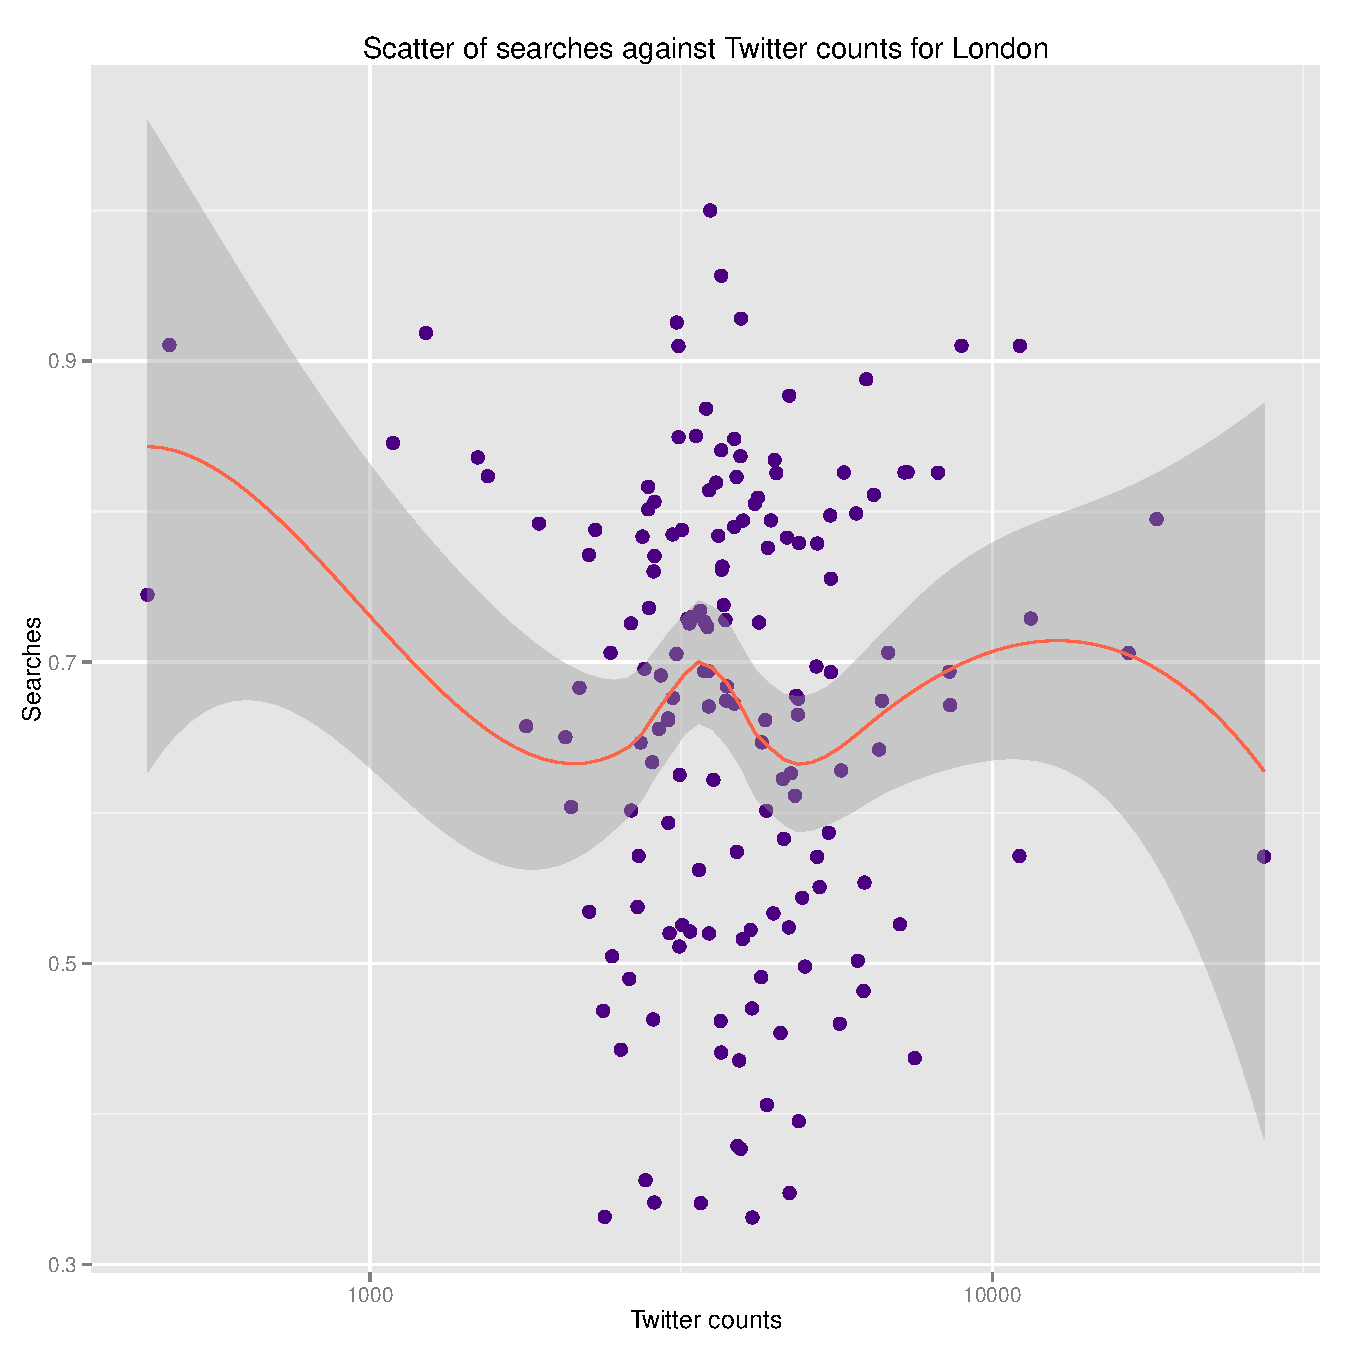
\includegraphics[width=65mm]{London} &   \includegraphics[width=65mm]{Sochi} \\
(a) London -- 0.003 & (b) Sochi -- 0.77 \\[6pt]
 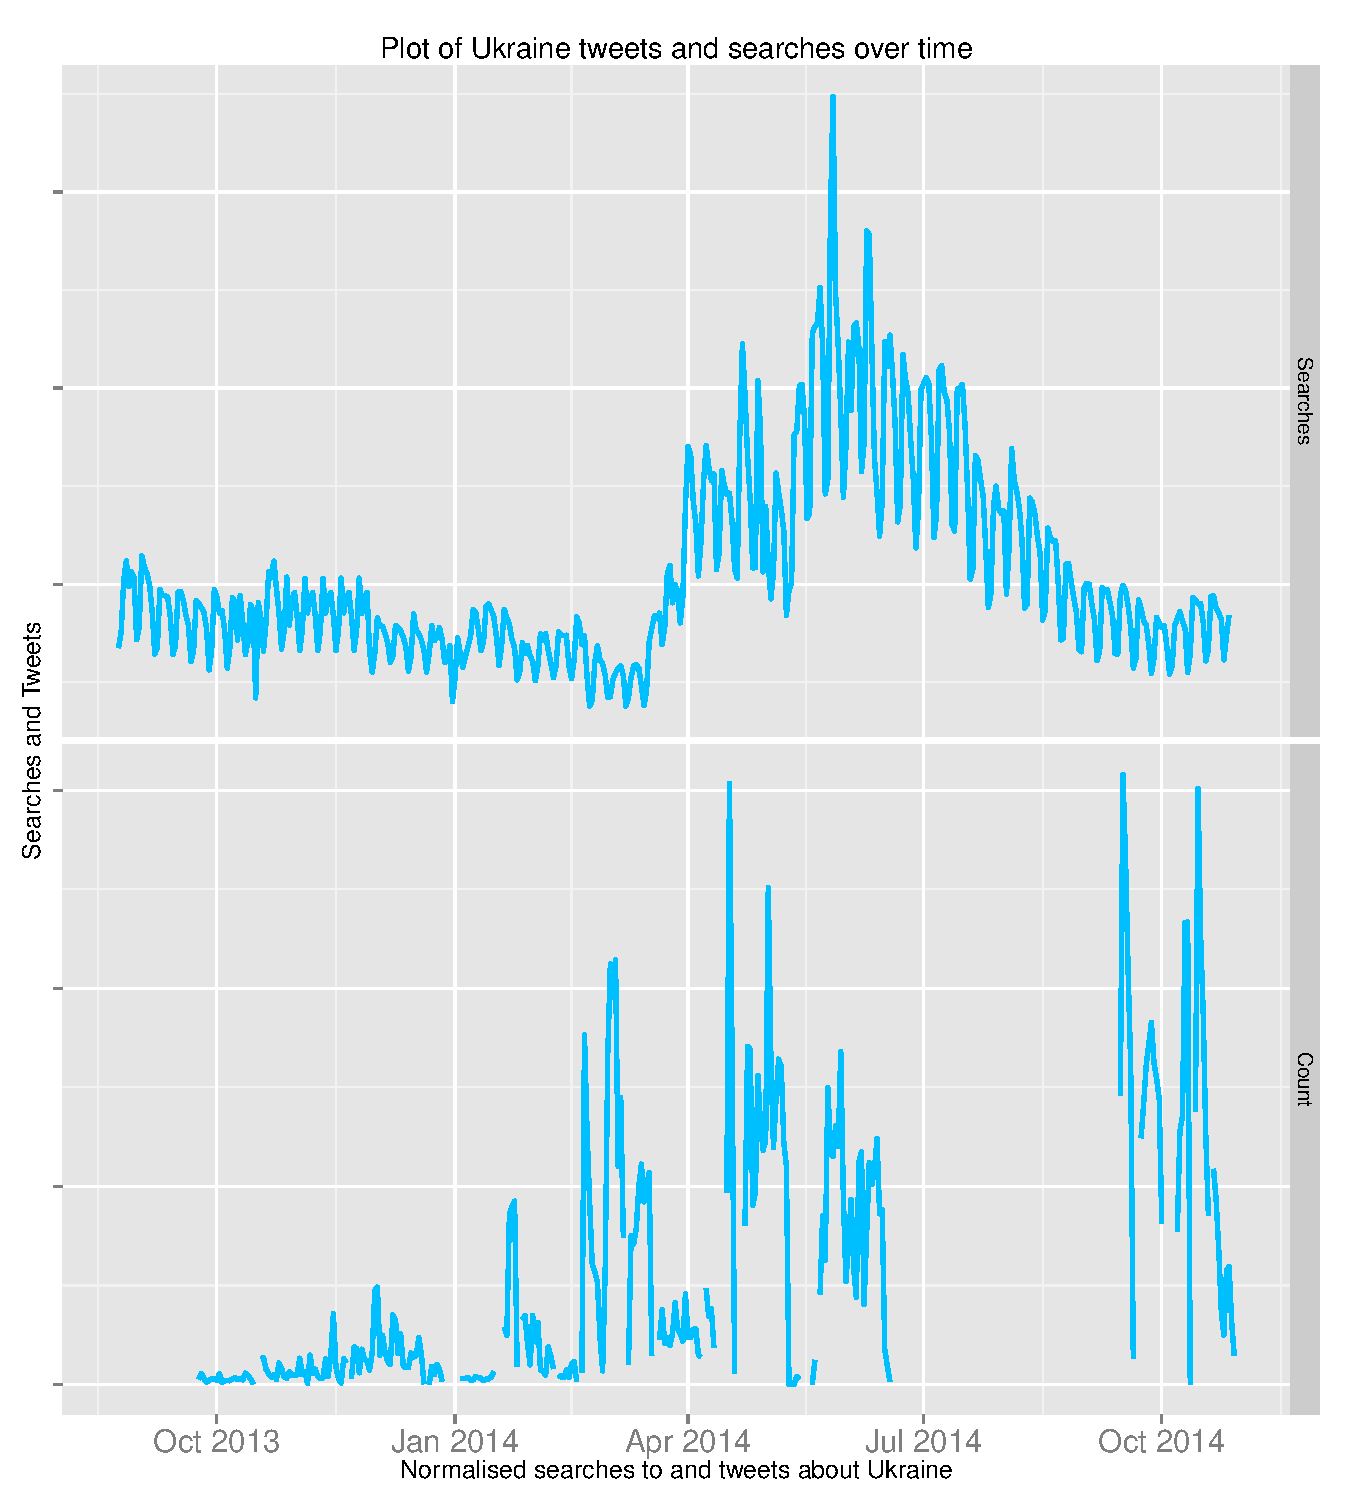
\includegraphics[width=65mm]{Ukraine} &   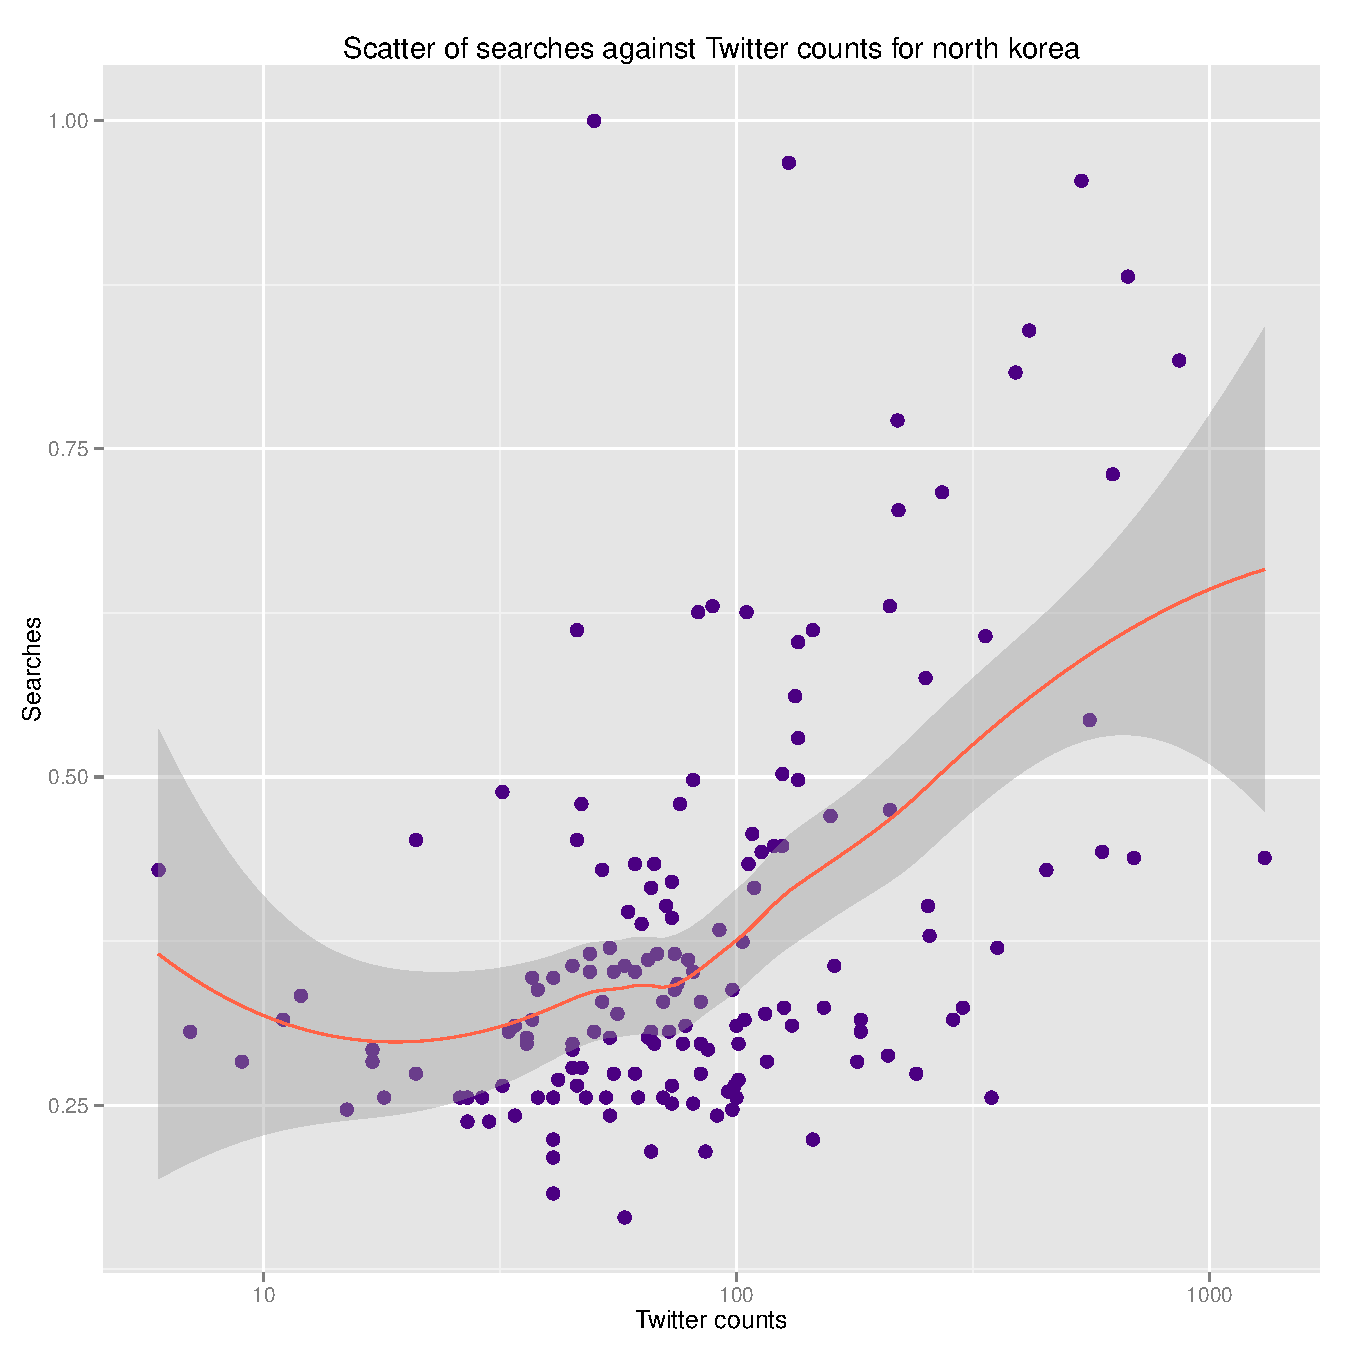
\includegraphics[width=65mm]{north-korea} \\
(c) Ukraine -- -0.36 & (d) North Korea -- 0.46 \\[6pt]
\end{tabular}
\caption{Scatter plots and correlation coefficients for 4 destinations- London, Sochi, Ukraine and North Korea. Those particular ones were picked because they each represent a separate class of destinations. London is a constant one and tweets don't influence the prediction. For Sochi the Olympiad has bumped the correlation coefficient up to 0.77, because people were tweeting and wanted to go and see the Olympiad. Ukraine is interesting, because the recent protests decreased the number of searches even though people were tweeting a lot, therefore the recent events made them less likely to want to go there. North Korea is an interesting outlier. Tourist to North Korea is quite a niche market and even though the sentiment is usually negative, people want to go there nonetheless. }
\end{figure}


All in all, 1282 of the places had an R value of less than 0.2 and the remaining 91 have a value of $>$ 0.2. A correlation of such small magnitude is not even worth reporting, however, since my task it not solely defined by predicting one attribute from another I wanted to include in order to give a perspective on the difficulty of the task. In Figure 4.3 there 4 examples of the subgroups of destinations. 


The best correlation is for Sochi, which has a correlation coefficient of 0.78. For Sochi we can observe at the top right a cluster of dates which have high volumes of tweets, but also a proportionally high number of searches. As we saw in Table \ref{tab:sochi-table} on page \pageref{tab:sochi-table} quite a few of the features picked out by the model were to do with the olympics - both the positive and the negative aspect. Interestingly enough, North Korea has got a similar profile, even though the correlation is not as strong. The correlation for Ukraine is very negative and so is for Kiev, both caused because of the recent problems in the country. What is really interesting would be to try to determine what causes the correlation to improve or what makes it worse. I did not have much time to work on that, but using some NLP techniques I believe it is entirely possible to be even more descriptive in what are the exact factors that influence it.


For those who have a value higher than 0.2 there is definitely some correlation, which could be pushed lower by all the outliers and holes in the data. Fixing that requires some cleansing of those holes in the data. I've described everything that I did for the cleansing in section \ref{sec:cleansing} on page \pageref{sec:cleansing}.


These results mean that there is a knock-on impact on the models that need to be used in order to perform the prediction. I wouldn't be able to fit an easy linear regression, because that will give predictions that are far from accurate. It also means that when doing the model I wouldn't be able to make one that works just with Twitter or the Twitter features. A hybrid method would be needed. One that is using past search data as a component as well in order to ensure that we are balancing out the weights of all the features, since the initial idea is to use Twitter as an exogenous factor with some weight. The best model that could do that job is LASSO \cite{lasso}. Due to the very fact that every place is quite different - apart from those with no correlation whatsoever - I fitted a model for each one and one for the overall searches and tweets, which can be found in more detail in chapter \ref{chap:model} on page \pageref{chap:model}.


\section{Data cleansing}
\label{sec:cleansing}


As I have previously mentioned there were two data source which I was using for this project - data obtained from the Twitter Streaming API and the Skyscanner search volumes. Even with one you can always experience some outages and problems. In this project there were a couple of sources of risk:
\begin{enumerate}
\item The script that collects data from the Streaming API - sometimes the API just wouldn't work. 
\item The searches data coming from Skyscanner being incorrect or partial - not spanning the full date range.
\end{enumerate}


The dates with incomplete or missing data can impact the regression negatively so it was vital to tidy up all of the data by either backfilling it or filling/removing the missing values. 

As far as the Skyscanner data set is concerned I have backfilled of data missing by using the Last 4 Fridays method in order to ensure that there are enough data point for carrying out all the tests. For the twitter counts, I have simply taken the mean for the values of missing Skyscanner data and dropped all the days where the Twitter collection had problems. For the full features I've just filled the missing values with 0, since there wasn't any better of filling those without removing all the hashtags and words that appear around a specific time and then disappear again.


\section{Feature extraction}


With the whole dataset ready for the statistical analysis I wanted to also extract some more features in order to check whether anything interesting will pop up - words that refer to particular events, etc. 


This was a very computationally intensive task and was probably the most difficult bit to get up and running without any major hiccups. What I did for this particular task was something quite similar to what is shown in Figure 2.2, however instead of just adding to the count of a place, I add to the counts of all the words that co-occur with the place name.  Pseudocode of the way it works is shown in Figure 2.4. The algorithm is simple enough, but the fact that dimensions of the count dictionary are massive I had to be extremely careful not to load up too much, because I experienced memory errors at the time of processing I decided to split them into partial counts and recombine those. 


\begin{figure}[]
\begin{center}
\begin{lstlisting}
place_names = get_all_placenames()

counts = {}
# Obtain all the counts
for file in twitter_data_files:
    for line in file:
        tweet = parse_json(line)
  
  	for place in place_names:
	    if place in tweet:
	        # split the text into words
                for token in tweet.split(' '): 
                    if token in one_word_placenames:
                        seen_place = True
                        counts[place][token][datetime] += 1

        if seen_place or travelWord:
            writeToFile(tweet)
            
# Recombination and output the final result

for place in place_names:
     data = load_file(feature_file)
     partial_counts = counts[place]
     data = data.append(partial_counts)
     # group them by the date time and then sum them up
     data.groupby('Datetime')
     data.sum()
     output(data)
    
\end{lstlisting}
\end{center}
\caption{Pseudocode for the filtering part. }
\end{figure}


Just in terms of numbers - for London I had 148877 features, so overall the data was the number of features times 160 dates, which had twitter place counts, feature counts and searches. All of that is then used as an input for the LASSO model, which removes the junk weights and assigns some weights to the non-junk features. It wasn't very easy working with the big sets, because in order to perform all of the predictions they all need to be held into memory, but thanks to Pandas \cite{pandas} the fitting and evaluation of those extended models takes about 2 hours, which is down from 6 without using CSVs and pandas data frames.


\section{Tools}


Every one of the aforementioned operations is performed in a separate Python class. The overall system can be separated into several subparts:
\begin{itemize}
\item Tools for extraction - FeatureExtractor, TwitterExtractor, HashtagExtractor;
\item Processing the data - SearchesProcessor, TwitterProcessor;
\item Tools for the shaping the data - Last4Backfill;
\item Models - LassoOverall, ExtendedLasso, LASSOClassifier;
\end{itemize}



\chapter{Models}
\label{chap:model}

\section{The baseline model}
\label{sec:baseline}

The baseline model for predicting the number of redirects Skyscanner has on a daily basis is called Last 4 Fridays. 
It works in the following way:
\begin{enumerate}
\item We want to predict the number of redirects/searches for this Friday.
\item We take the number of redirects/searches Friday from last week, the week before, etc, until we have the counts form the previous 4 weeks for the corresponding day.
\item We then assign weights to those 4 numbers and assign weights -- the most recent one will get the highest weight, the one after about a half and so on. The exponential weighting scheme captures short term seasonality.
\end{enumerate}

This model was tested out against more complex models like ARIMA and Autoregressive Vector Methods and it performed really well, but unlike the others it was many times simpler to program and maintain.

\section{Last 4 Fridays + Twitter Counts}

The first model I build was not a radical new approach, but rather an increment on the previous one.

I generated a list of tuples which contained the following information:
\begin{itemize}
\item Twitter count for the place -- how many times it was mentioned in conjunction with a travel term.
\item Same day of the week from last week
\item Same day of the week from 2 weeks ago
\item Same day of the week from 3 weeks ago
\item Same day of the week from 4 weeks ago
\end{itemize}

What this is is a version of Last 4 Fridays which now has Twitter Counts. Instead of using the exponential weights from the previous algorithm I let LASSO determine their weights.
With LASSO I had weights for each of the 272 cities. After measuring the RMSEs for the L4F algorithm and expanded version with Twitter Counts the former performs better on 193 of the 272 cities. In the top 10 L4F+Twitter performs better on 2 out of 10. 

Dublin which is in the 4th spot in terms of volumes is quite interesting. I plotted out the counts against searches just to see how it looks:
%
%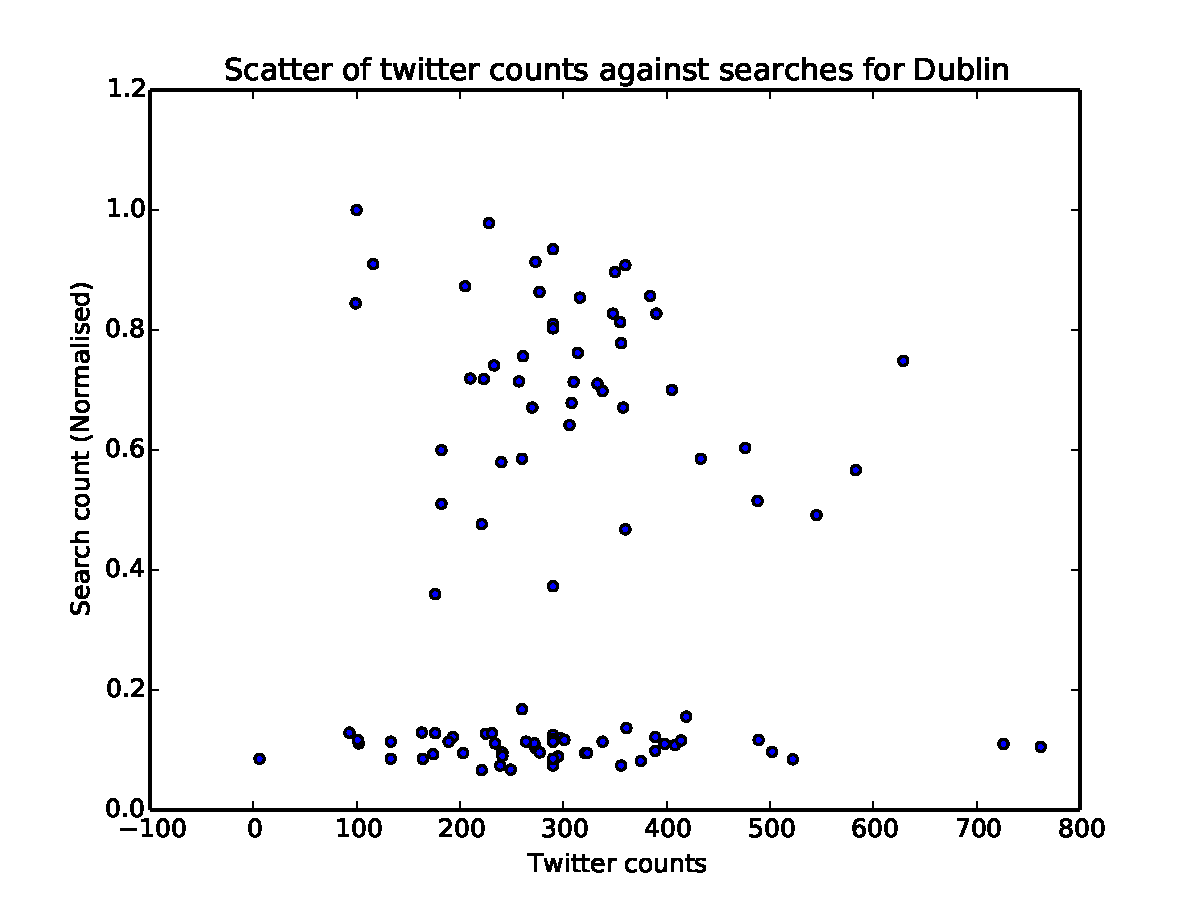
\includegraphics[width=\textwidth]{Dublin}  
%
%\newpage
\section{Results}

And here are the results for the top 10 destinations by volume (they have the highest RMSEs).

\begin{tabular}{ l | r | r }
City	& RMSE L4F+Twitter &RMSE L4F \\
\hline
London & 3335.869525 & 3160.05886 \\
Paris	 & 939.1057276 & 921.6785638  \\
Barcelona & 920.6831066 & 897.6473097  \\
Milan & 760.3436591 & 760.9286718  \\
Rome & 710.7052517 & 705.8388511  \\
Manchester & 574.8431422 & 572.4116201  \\
Dublin & 514.584231	 & 527.884409  \\
Amsterdam & 550.2254781 & 516.2054596  \\
Tenerife & 544.6187529 & 502.0270723  \\
Moscow & 499.1803266 & 495.2139406  \\
\end{tabular}


This is quite a good start considering the fact that all the weights were automatically determined by the LASSO algorithm and the fact that I have only about 130 data points so far (130 days).

\section{Future improvements}

The next on the list is to expand the feature set with more features from Twitter such as:


\begin{itemize}
\item Specific words.
\item Trending event or not.
\item Investigate whether sentiment will be useful here.
\end{itemize}

With those I'll be able to better the model and reduce the RMSE across the whole board and hopefully beat the current prediction algorithm for more than 80\% of the examples.

\chapter{Results}


Due to the lack of any research in this particular area setting the objectives for this project was very difficult. Planning on how to approach and tackle was in itself a challenge. There is no current proposed method of doing this, so there was no gold standard against which I could benchmark my trained models. That made it particularly hard to see whether the model is right or wrong and what should I strive to beat.


To get started, I needed to understand the data better and ask myself what I am trying to achieve. As mentioned in the introduction there are two main types of destinations:

\begin{itemize}
\item One that have a constant search volume to them which doesn't change too much over the course of the year - those are the big cities such as London, New York, Paris and to some extent the searches to some countries. 
\item Smaller places such as Ibiza, Alicante, Faro and more exotic destinations such as Lusaka, Tobago and many others that have highly seasonal demand.
\end{itemize}
The difference in the two is graphically represented on the next page in Figure \ref{london-searches} and \ref{ibiza-searches}. 

\begin{figure}[]
\begin{center}
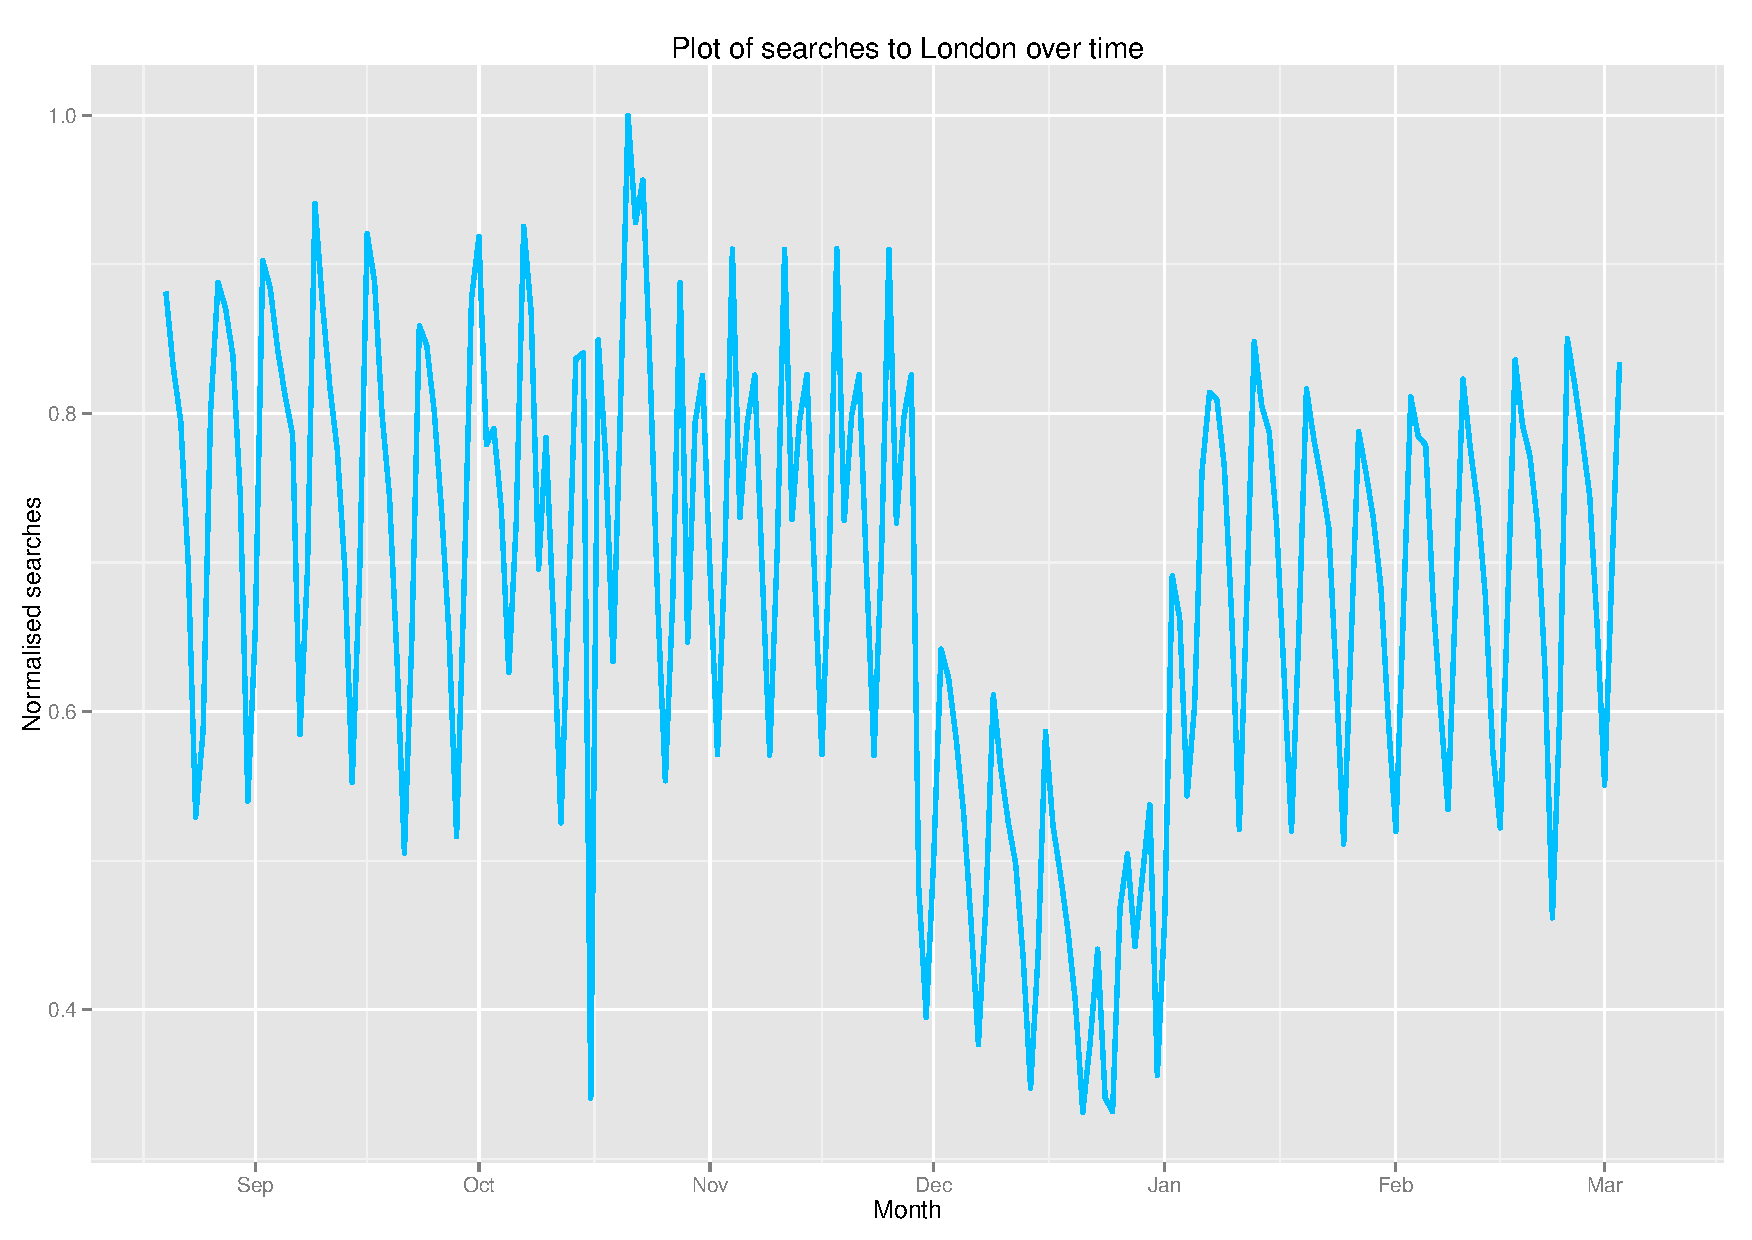
\includegraphics[scale=0.4]{london-searches}
\end{center}
\caption{Searches to London - as we can see the trundling is going to be almost parallel to the X axis.The slight dip in December is due to seasonality. That is noticed across the industry as a whole}
\label{london-searches}
\end{figure}


\begin{figure}[]
\begin{center}
\includegraphics[scale=0.4]{ibiza-searches}
\end{center}
\caption{Searches to Ibiza - in this plot we can get the idea of seasonality. The dips is observed as soon as enter autumn and then in January the searches to such destinations pick up again as people are starting to plan their summer holidays}
\label{ibiza-searches}
\end{figure}

Naturally, because of the constant and not so changing nature of the first group, I would expect my model to perform better on the second group. The Root Mean Squared Error from my models on the 2nd group should be smaller or roughly the same as the error generated by the in-house algorithm. It's called  "Last 4 Fridays" and essentially it is a slightly tweaked version of an exponentially weighted moving average, which takes into account seasonality. A more detailed discussion as to why this was picked as the baseline can be found in Chapter \ref{sec:baseline} on page \pageref{sec:baseline}.


\section{Results for the first iteration of the algorithm}


In order to get started with this problem and generate a first set of results I had to identify a good way of modelling the problem and how to predict the output from some inputs. The first way of doing it suggested by my supervisor was to use LASSO \cite{lasso} in order to determine the weights for all of my inputs. 


The way the first iteration of my model works is the following - for every day you take the same day the week before, the week before that and so on for the last 4 weeks and you also take the Twitter counts for a destination as a feature as well. Instead of fixing their weights as in the in-house algorithm, I chose to let LASSO pick the weights for every feature. This way we get an incremental improvement over the Last 4 Fridays, that is taking into account one of the many exogenous factors that could influence the search volumes either upwards or downwards. I expected that to yield better results for the 2nd group of destinations and possibly for some from group 1. I will refer to the first iteration of the model as TwitterDF, where DF stands for dynamic Fridays. 


Overall, I was very pleasantly surprised by the results. On the full set of 1372 destinations, the first iteration of my model generated better predictions and had lower RMSE on 1034 of the destinations. On the other hand the in-house champion Last 4 Fridays performed better on 338 of the destinations. In order to illustrate that difference there is a scatter plot of the RMSEs in Figure \ref{rmse-scatter}. That means that my model is better on 75.3\% of all the destinations.

\begin{figure}[]
\begin{center}
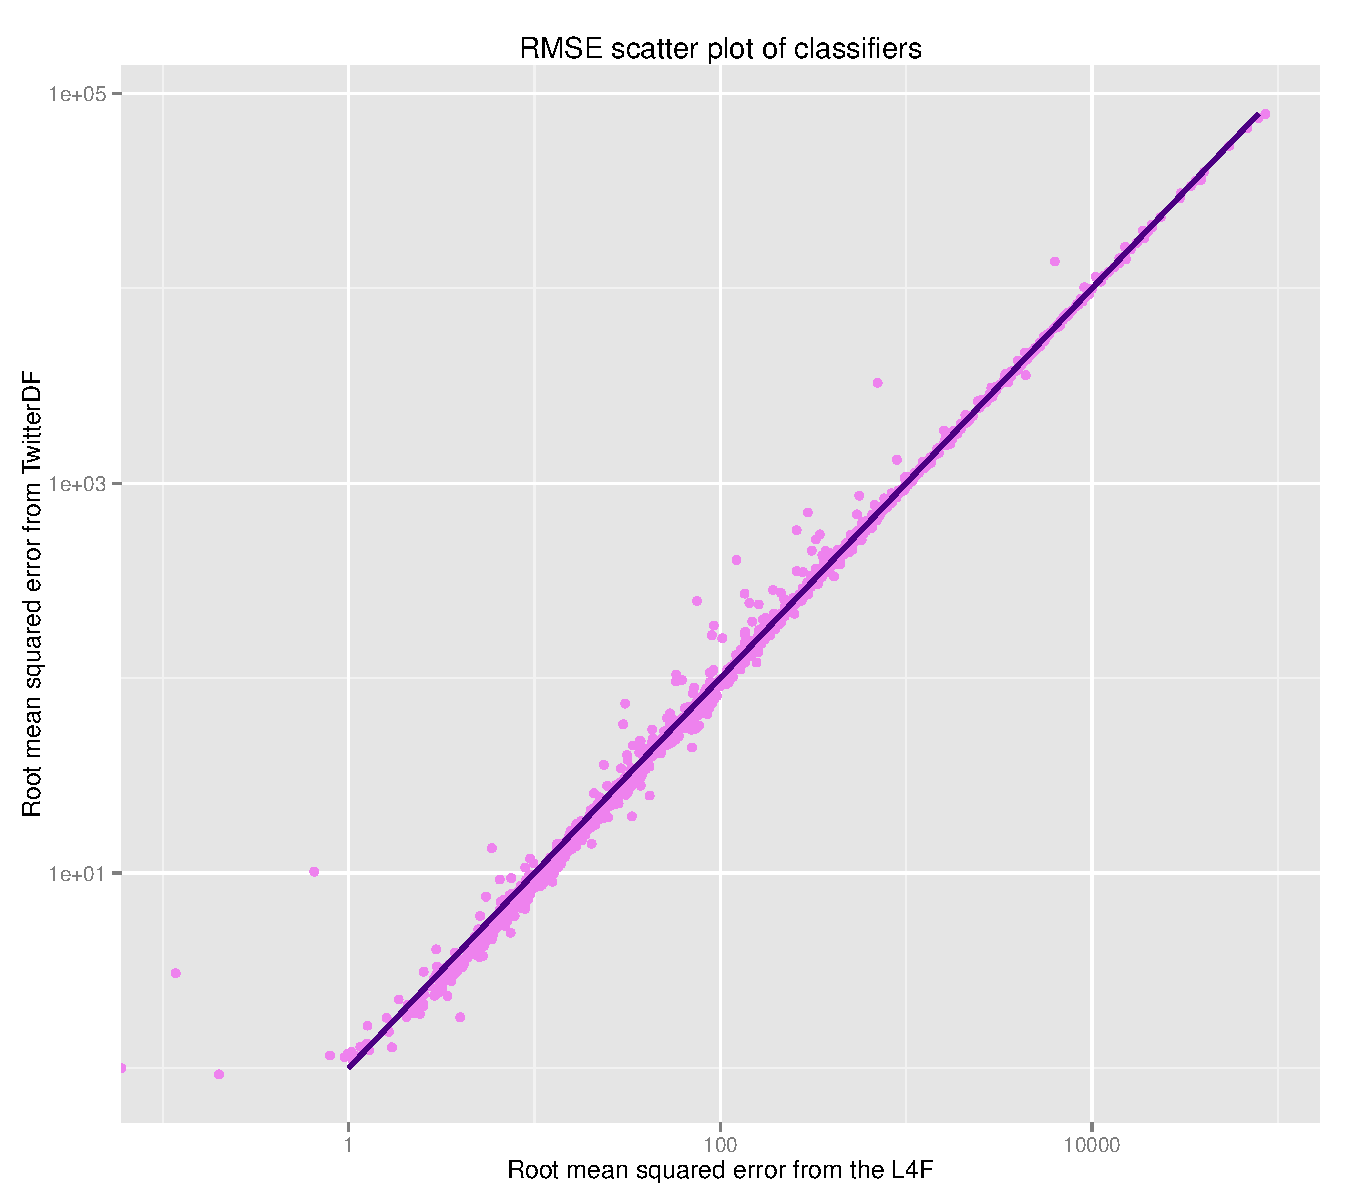
\includegraphics[scale=0.4]{RMSE}
\end{center}
\caption{Scatter plot of the RMSE of TwitterDF model and Last 4 Fridays. To put things into perspective, I've also plotted the y=x line to make it easier to visualise the border between the two. Anything below the line is where my model performs better and anything above L4F.  }
\label{rmse-scatter}
\end{figure}

In Figure \ref{rmse-scatter} we can see that the performance of the the models is actually quite similar. Almost all of the dots are distributed along the x=y line. Contrary to my expectations that destinations from group 2 would be better classified by my model, actually it performs just as well on the more constant ones from group 1. 

In Table \ref{4-1} and \ref{4-2} you can find some picked which illustrate the worst performing models and best performing ones in order to give an illustration of what is the improvement and degradation of performance.

\begin{table}[]
\begin{center}
\begin{tabular}{ l | r | r | r}
Place & RMSE L4F & RMSE Twitter & Improvement \\
\hline
Parkersburg & 3.99 & 1.82 & 54.38\% \\
Bismarck & 33.41 & 19.53 & 41.54\% \\
Marshall Islands & 41.63 & 24.99 & 39.98\% \\
Cayo Coco & 70.44 & 44.10 & 37.38\% \\
Yakima & 7.44 & 4.94 & 33.65\% \\
Jonesboro & 3.40 & 2.34 & 31.11\% \\
Casper & 20.30 & 14.14 & 30.34\% \\
Barrow & 5.28 & 3.76 & 28.81\% \\
Niue & 12.50 & 9.02 & 27.82\% \\
Cedar City & 5.08 & 3.71 & 26.91\% \\
Sudbury & 8.89 & 6.56 & 26.24\% \\
\end{tabular}
\end{center}
\caption{Results for destinations that yielded the best improvement in percentage terms when classified with the model from this project in comparison to the in-house one. As we can see they are fairly small niche destinations where it seems that people tweeting about it likely to result in a flight search to that place.}
\label{4-1}
\end{table}

\begin{table}[]
\begin{center}
\begin{tabular}{ l | r | r | r}
Place & RMSE L4F & RMSE Twitter & Improvement \\
\hline
Hayman Island & 0.12 & 3.06 & -2511.33\% \\
Airlie Beach & 0.65 & 10.17 & -1456.42\% \\
Venezuela & 701.98 & 3277.16 & -366.85\% \\
Crooked Creek & 0.20 & 0.93 & -362.78\% \\
Pereira & 74.94 & 248.77 & -231.97\% \\
Launceston & 122.28 & 404.13 & -230.49\% \\
Jodhpur & 30.80 & 74.05 & -140.40\% \\
Manaus & 295.66 & 707.50 & -139.30\% \\
Del Rio & 5.89 & 13.42 & -127.63\% \\
Trondheim & 257.36 & 573.07 & -122.68\%
\end{tabular}
\end{center}
\caption{Results for destinations that yielded the biggest negative improvement. Quite an interesting mix destinations. The Venezula result is attributed to Venezuela trending lately, because of the civil uprisings. Eliminating such "negative" influences is one of my goals for next year.}
\label{4-2}
\end{table}


If we look at the top 10 destinations in terms of RMSE (and in flight searches) in Table \ref{top10} we see something quite surprising.  The improvement is positive in 9 out of the 10 examples. Even though it's small, the very fact that there is an improvement, means that taking into account exogenous factors is beneficial and can contribute positively to the quality of the prediction.

\begin{table}[]
\begin{center}
\begin{tabular}{ l | r | r | r}
Place & RMSE L4F & RMSE TwitterDF & Improvement \\
\hline
Spain & 85,844 & 78,424 & 8.64 \% \\
United States & 78,480 & 74,782 & 4.71\% \\
United Kingdom & 68,706 & 66,335 & 3.45\% \\
Italy & 54,804 & 53,780 & 1.87\% \\
London & 40,129 & 39,554 & 1.43\% \\
Russia & 38,712 & 36,033 & 6.92\% \\
Germany & 36,113 & 35,672 & 1.22\% \\
France & 34,020 & 33,393 & 1.84\% \\
Thailand & 29,997 & 30,701 & -2.34\% \\
Turkey & 29,616 & 28,912 & 2.38\% 
\end{tabular}
\end{center}
\caption{Results for the top destinations by RMSE of L4F. 9/10 have lower RMSEs with TwitterDF. As we can see for the top destination - Spain - the improvement is 8.64\%, which is great, because I expected the model to perform worse on places from group 1.}
\label{top10}
\end{table}


\newpage
\section{Results for the 2nd iteration}

The 2nd iteration, was to fix the weights of the last 4 fridays and use the exponential weighting scheme that we have in the L4F model. I called that model TwitterCF where CF stands for compound Fridays. The scatter comparison for the two models is in Figure \ref{rmse_scatter_by_reg}. In Table \ref{comparison-all} is the overall comparison of which model has the lowest RMSE for how many of the total models. 

\begin{figure}[h!]
\begin{center}
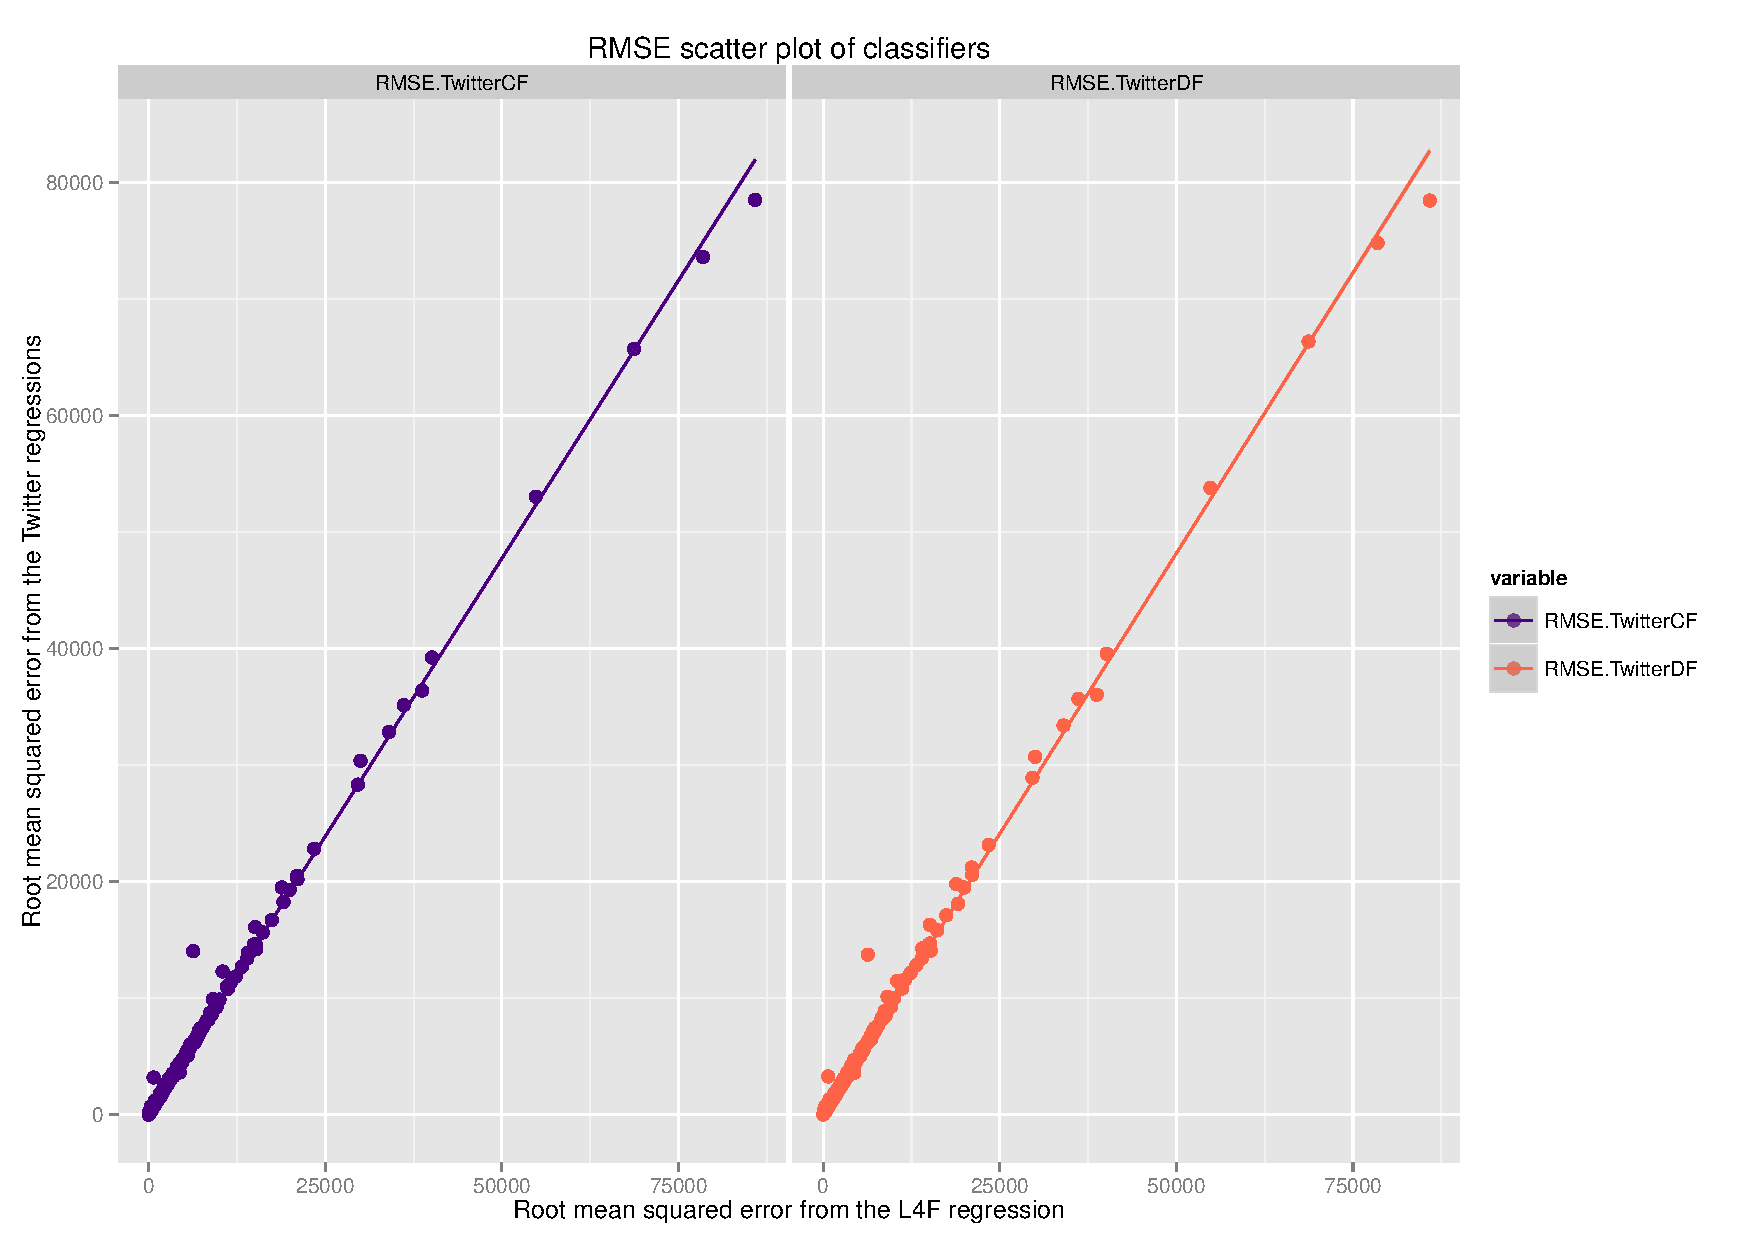
\includegraphics[scale=0.4]{rmse_scatter_by_reg}
\end{center}
\caption{The two models compared. TwitterCF stands for compound Friday - taking all of the previous Fridays with predetermined weights and using them as a single weight in the regression. TwitterDF is leaving everything to LASSO.}
\label{rmse_scatter_by_reg}
\end{figure}

\begin{table}[h!]
\begin{center}
\begin{tabular}{ l | r }
Method & NumBest \\
\hline
L4F & 226 \\
TwitterCF & 741 \\
TwitterDF & 405 \\
\hline
\textbf{Total} & \textbf{1372}
\end{tabular}
\end{center}
\caption{Comparison of the three methods and who had the best results on the dataset of 1372 points. As we can see, the Twitter models have got a definite majority. 83\%+ of the results have the lowest RMSE with the Twitter models}
\label{comparison-all}
\end{table}

In Table \ref{big-table} you can find a more detailed breakdown of the top 20 destinations by RMSE for L4F sorted descending. It includes the improvement of the Twitter models and the improvement of the CF model over the DF one. Overall, the average improvement of the CF model is 0.96\% across all the 1372 individuals models for every destination.

\begin{table}[p]
\begin{center}
\begin{tabular}{ l | r | r | r | r | r | r }
Place & L4F &  TwitterCF & TwitterDF & Best & Improv. & CF/DF Imp. \\
\hline
Spain & 85,844 & 78,485 & 78,424 & TDF & 8.64\% & -0.08\%\\
US & 78,480 & 73,581 & 74,782 & TCF & 6.24\% & 1.61\%\\
UK & 68,706 & 65,696 & 66,335 & TCF & 4.38\% & 0.96\%\\
Italy & 54,804 & 53,020 & 53,780 & TCF & 3.26\% & 1.41\%\\
London & 40,129 & 39,222 & 39,554 & TCF & 2.26\% & 0.84\%\\
Russia & 38,712 & 36,375 & 36,033 & TDF & 6.92\% & -0.95\%\\
Germany & 36,113 & 35,137 & 35,672 & TCF & 2.70\% & 1.50\%\\
France & 34,020 & 32,816 & 33,393 & TCF & 3.54\% & 1.73\%\\
Thailand & 29,997 & 30,374 & 30,701 & L4F & -1.26\% & 1.07\%\\
Turkey & 29,616 & 28,316 & 28,912 & TCF & 4.39\% & 2.06\%\\
Greece & 23,423 & 22,810 & 23,144 & TCF & 2.62\% & 1.44\%\\
Australia & 21,072 & 20,189 & 20,573 & TCF & 4.19\% & 1.86\%\\
New York & 21,026 & 20,498 & 21,198 & TCF & 2.51\% & 3.30\%\\
Paris & 19,966 & 19,287 & 19,492 & TCF & 3.40\% & 1.05\%\\
Barcelona & 19,087 & 18,237 & 18,093 & TDF & 5.21\% & -0.80\%\\
Bangkok & 18,831 & 19,496 & 19,783 & L4F & -3.53\% & 1.45\%\\
Portugal & 17,429 & 16,694 & 17,103 & TCF & 4.22\% & 2.39\%\\
Netherlands & 16,146 & 15,638 & 15,816 & TCF & 3.14\% & 1.12\%\\
China & 15,212 & 14,188 & 14,074 & TDF & 7.48\% & -0.81\%\\
Istanbul & 15,121 & 14,642 & 14,692 & TCF & 3.16\% & 0.34\%
\end{tabular}
\end{center}
\caption{Comparison of the RMSE generated by the 3 models for the first 20 destinations with highest RMSE for L4F. The Best column indicates who has the lowest RMSE for that destination. Out of the twenty TwitterDF and TwitterCF perform better on 18 of the destinations. The overall numbers can be found in table 2.4. The average improvement of CF over DF is 0.96\%, which even though small is significant nonetheless. }
\label{big-table}
\end{table}

%\section{Results when shifting by one day}

\newpage
\section{Results for the algorithm with more features}
\label{sec:features}

In the next iteration of the model I didn't limit it to just twitter counts and searches from previous dates. For this particular model I've used all the words co-occurring with a place name as features. Of course, there is a lot of junk, so I removed all the emoji characters and all the stop words in order to prevent overwhelming the LASSO with a lot of junk features.

In Table \ref{table-tenerife}, \ref{table-sochi} you can see the results from the extended model on Tenerife and Sochi. In the tables you can see the improvement in RMSE for Twitter and the decrease in the number of features with non-zero weights. For both of those destinations, the Twitter models perform better for some values of the penalisation parameter $\alpha$. I've picked them, because they are both really interesting - for Tenerife L4F start well, then Twitter has lower RMSE, but as we discard more and more features, L4F wins again. Sochi was picked because of the olympics, which has massively affected the number of searches to Sochi (increase of about 10 times), but the number of tweets about Sochi has gone up as well. 
It's also quite interesting, because of local minima of RMSR, where it decreases and then picks up again.

\begin{table}[h]
\begin{center}
\begin{tabular}{ l | r | r | r | r | r | r}
$\alpha$ & $>$ 0 W CF & RMSE TCF & $>$ 0 W DF & RMSE TDF & RMSE L4F & Best\\
\hline
0.50 & 191 & 11,683 & 200 & 14,961 & 1,517 & L4F\\
1 & 175 & 12,507 & 177 & 15,647 & 1,517 & L4F\\
2 & 146 & 13,288 & 151 & 15,161 & 1,517 & L4F\\
5 & 136 & 13,607 & 131 & 14,387 & 1,517 & L4F\\
10 & 116 & 12,728 & 114 & 11,341 & 1,517 & L4F\\
20 & 112 & 11,379 & 108 & 8,950 & 1,517 & L4F\\
50 & 88 & 6,601 & 85 & 5,197 & 1,517 & L4F\\
125 & 51 & 1,946 & 56 & 2,009 & 1,517 & L4F\\
250 & 33 & 1,684 & 36 & 1,788 & 1,517 & L4F\\
\hline
500 & 22 & 1,596 & 23 & 1,465 & 1,517 & TDF\\
1,000 & 11 & 1,423 & 13 & 1,593 & 1,517 & TCF\\
2,000 & 5 & 1,356 & 8 & 1,815 & 1,517 & TCF\\
4,000 & 1 & 1,366 & 4 & 1,854 & 1,517 & TCF\\
8,000 & 1 & 1,366 & 4 & 1,853 & 1,517 & TCF\\
16,000 & 1 & 1,366 & 4 & 1,852 & 1,517 & TCF\\
32,000 & 1 & 1,366 & 4 & 1,850 & 1,517 & TCF\\
\end{tabular}
\end{center}
\caption{Improvement in RMSE for Tenerife. As we can see after we get to a certain point the Twitter models get better and better, until it gets to discarding all of the weights, but the Fridays. The optimal result for Twitter CF is with 5 weights, since the reduction in RMSE afterward is negligible, while the DF version performs best with 23 and it starts getting worse. The features and weights at $\alpha = 1000$ are in Table 4.7}
\label{table-tenerife}
\end{table}

\begin{table}
\begin{center}
\begin{tabular}{l | r}
Feature & Weight \\
\hline
time & 583.35 \\
\#tenerife & -87.43 \\
\#solareclipse & 35.74\\
tenerife & -19.29\\
friend & 64.81\\
Fridays & 0.75\\
begins & -30.50\\
heres & 7.72\\
would & -273.96\\
canary & -7.56\\
view & -10.86 \\
\end{tabular}
\end{center}
\caption{Weights for Tenerife at $\alpha=1000$. These are the weights that the TwitterCF model has picked.}
\end{table}

\begin{figure}[]
\begin{center}
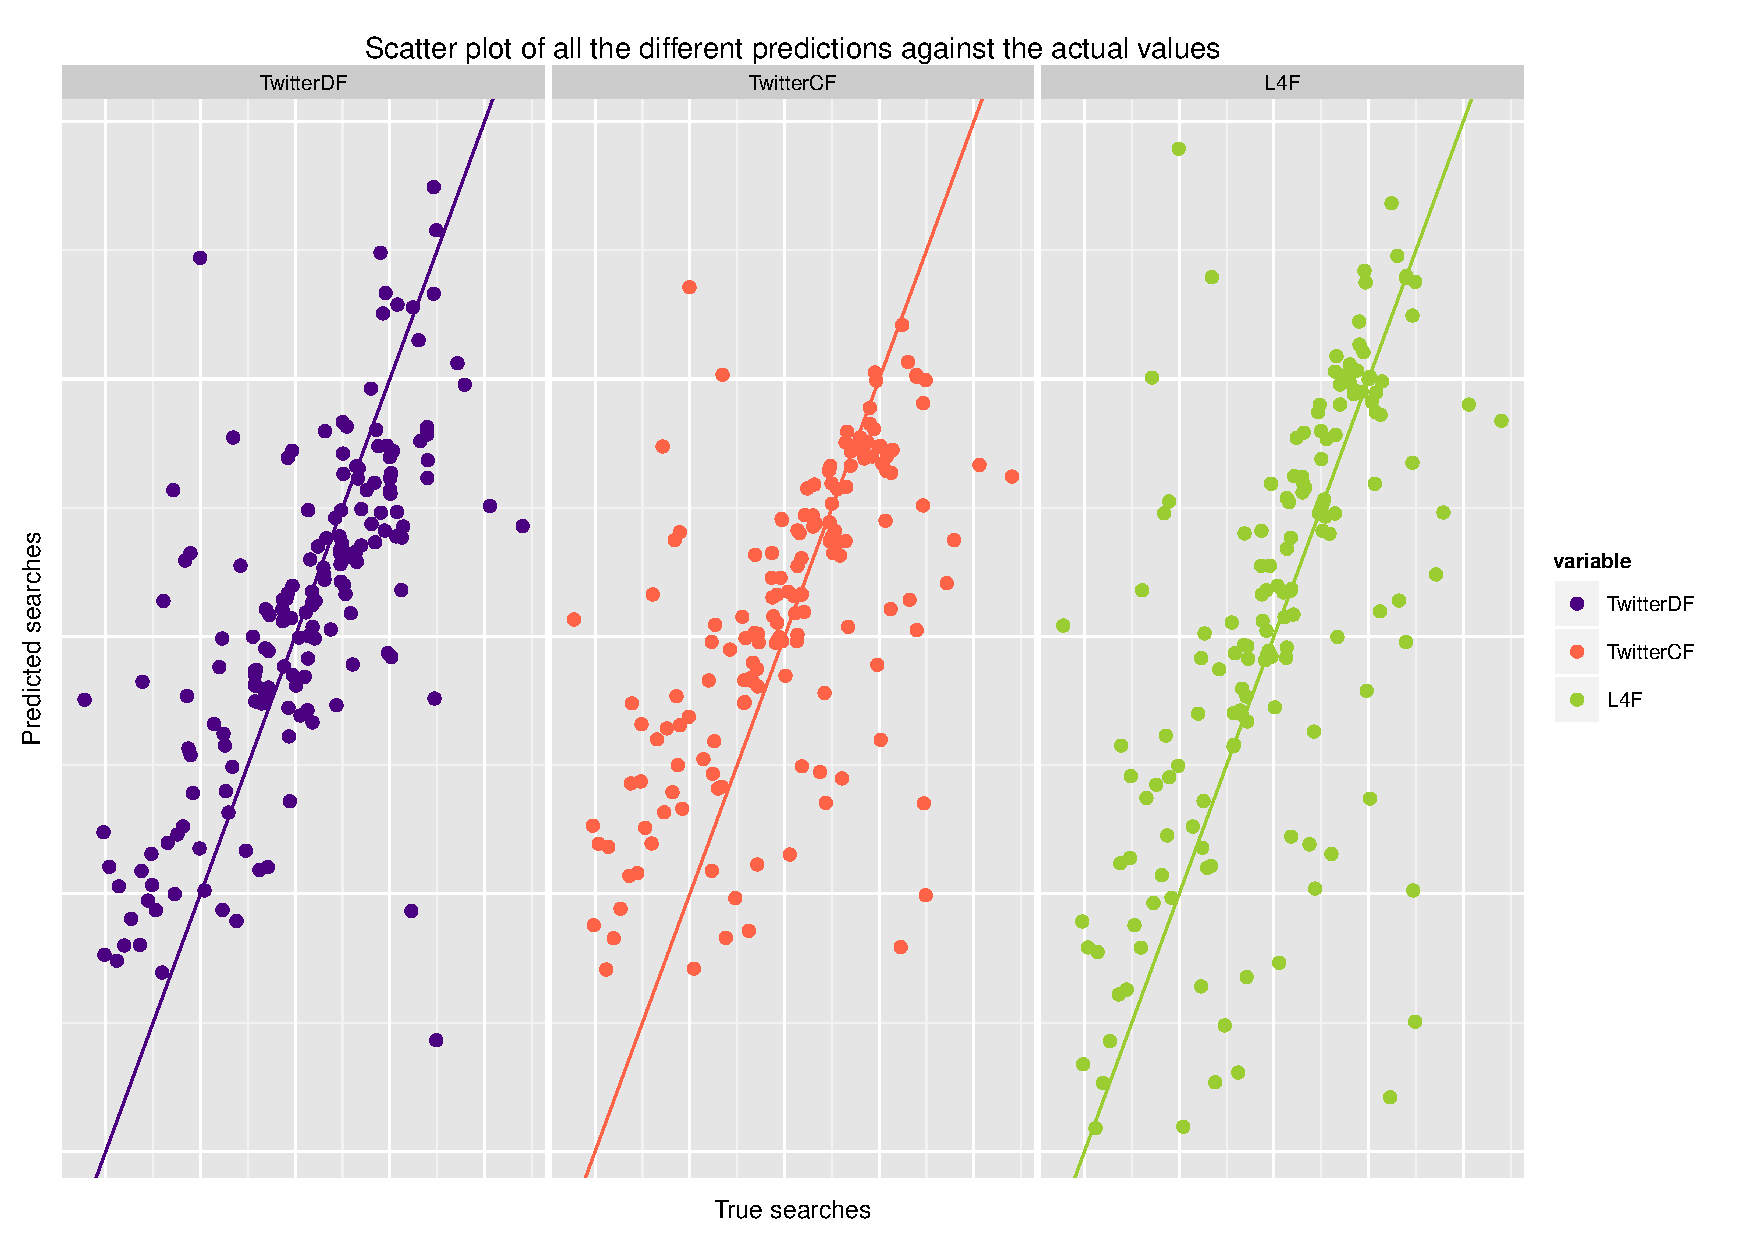
\includegraphics[scale=0.5]{plots/Tenerife}
\end{center}
\caption{Predictions vs actual for a destination from group 2 - Tenerife. For this group Twitter models make actual gains, albeit small.}
\end{figure}

\begin{table}[h!]]
\begin{center}
\begin{tabular}{ l | r | r | r | r | r | r}
$\alpha$ & $>$ 0 W CF & RMSE TCF & $>$ 0 W DF & RMSE TDF & RMSE L4F & Best\\
\hline
0.5 & 268 & 10,545 & 377 & 15,909 & 9,156 & L4F\\
1 & 200 & 10,505 & 260 & 15,108 & 9,156 & L4F\\
2 & 170 & 9,976 & 192 & 13,693 & 9,156 & L4F\\
\hline
5 & 138 & 8,774 & 158 & 10,720 & 9,156 & TCF\\
10 & 126 & 8,964 & 132 & 9,808 & 9,156 & TCF\\
20 & 112 & 9,051 & 115 & 10,802 & 9,156 & TCF\\
50 & 99 & 8,867 & 101 & 9,577 & 9,156 & TCF\\
125 & 81 & 9,129 & 82 & 8,604 & 9,156 & TDF\\
250 & 60 & 8,924 & 57 & 8,304 & 9,156 & TDF\\
500 & 41 & 8,335 & 44 & 7,982 & 9,156 & TDF\\
1,000 & 29 & 8,443 & 28 & 8,164 & 9,156 & TDF\\
2,000 & 16 & 8,424 & 19 & 8,341 & 9,156 & TDF\\
4,000 & 7 & 9,143 & 9 & 9,307 & 9,156 & TCF\\
\hline
8,000 & 3 & 9,759 & 6 & 9,938 & 9,156 & L4F\\
16,000 & 2 & 9,727 & 5 & 9,860 & 9,156 & L4F\\
32,000 & 2 & 9,950 & 4 & 10,010 & 9,156 & L4F\\
\end{tabular}
\end{center}
\caption{Improvement in RMSE with the expanded feature set for Sochi, which is in 2nd group of destinations.  
As you can see in terms of absolute value, the RMSE for the Twitter model with compound fridays - RMSE TCF - has decreased 20\% for the area where TCF has the lowest RMSE. I have separated the area where the Twitter Models are better with two horizontal lines. The RMSE for TDF is 2 times lower at $\alpha=500$ and that's where the model performs the best. Both models have a comparable number of weights, which is really interesting.}
\label{table-sochi}
\end{table}

\begin{table}[]
\begin{center}
\begin{tabular}{l | r}
Feature & Weight\\
\hline
team & 16.08\\
\#olympics2014 & 2.40\\
Count & 1.34\\
olympic & 1.30\\
Friday1 & 0.75\\
canada & 0.72\\
Friday3 & 0.16\\
Friday2 & 0.11\\
Friday4 & -0.15\\
hotel & -1.07\\
\#seeyouinsochi & -1.22\\
jump & -1.49\\
\#olympics & -2.24\\
dog & -2.56\\
sochi & -2.52\\
\end{tabular}
\end{center}
\caption{Handpicked features for Sochi at $\alpha=500$. The total number of features is 44 and they are the ones picked by TwitterDF. Interestingly enough dog, sochi and hotel very negative weights. On the other hand there are a few positive weights that relate to the olympics.} 
\label{tab:sochi-table}
\end{table}



\begin{figure}[]
\begin{center}
\includegraphics[scale=0.5]{plots/Sochi}
\end{center}
\caption{Predictions vs actual for a destination for Sochi. The olympics made any pattern in the data very hard to spot.}
\end{figure}

As we can see the more the junk features are penalised the classification improves. However that is still just the beginning. Next year I will apply more NLP on the Twitter dataset trying to capture only the relevant tweets that will result in an improvement of the overall RMSE for the classifier. 


\begin{figure}[]
\begin{center}
\includegraphics[scale=0.4]{Sochi}
\end{center}
\caption{Searches and tweets to Sochi. The massive spike is around the Olympics. As we can see the two time series are correlated and the spike it tweets is just a bit before the spike in searches.}
\end{figure}


However those gains are not observed across the whole board at all. In Table \ref{uk} are the results for the United Kingdom. Even though we notice a  very significant improvement, the results are still poorer than L4F. Of course, there are still 14 and 11 weights in both models, so we could continue increasing the penalisation factor further, but that would turn tweaking and tuning the classifiers into a very complicated and laborious task and of course we will get into the problem of overfitting.

\begin{table}[]
\begin{center}
\begin{tabular}{ l | r | r | r | r | r | r}
$\alpha$ & $>$ 0 W CF & RMSE TCF & $>$ 0 W DF & RMSE TDF & RMSE L4F & Best\\
\hline
0.5 & 583 & 60,924 & 649 & 70,068 & 8,700 & L4F\\
1 & 467 & 65,234 & 523 & 68,728 & 8,700 & L4F\\
2 & 369 & 65,253 & 412 & 76,945 & 8,700 & L4F\\
5 & 280 & 59,667 & 290 & 69,158 & 8,700 & L4F\\
10 & 231 & 54,972 & 241 & 62,057 & 8,700 & L4F\\
20 & 197 & 58,161 & 212 & 55,629 & 8,700 & L4F\\
50 & 167 & 62,001 & 175 & 77,956 & 8,700 & L4F\\
125 & 147 & 59,146 & 155 & 90,270 & 8,700 & L4F\\
250 & 139 & 73,864 & 142 & 105,197 & 8,700 & L4F\\
500 & 116 & 81,806 & 120 & 96,173 & 8,700 & L4F\\
1,000 & 106 & 84,796 & 110 & 91,576 & 8,700 & L4F\\
2,000 & 98 & 61,891 & 94 & 60,692 & 8,700 & L4F\\
4,000 & 71 & 44,306 & 68 & 61,037 & 8,700 & L4F\\
8,000 & 44 & 56,021 & 43 & 49,030 & 8,700 & L4F\\
16,000 & 27 & 31,209 & 29 & 28,339 & 8,700 & L4F\\
32,000 & 11 & 15,895 & 14 & 16,034 & 8,700 & L4F\\
\end{tabular}
\end{center}
\caption{Expanded features for the United Kingdom. We don't notice the same gain here. Both TwitterDF and CF decrease the number of features significantly the RMSE for both is about 2x times the one for L4F.}
\label{uk}
\end{table}

\newpage
\section{Results on the full dataset}

%\subsection{With just Twitter counts}

Another interesting benchmark was how it performs on the overall search volumes. In Table 4.11 you will find how the two models perform on the all the Twitter counts summed together and the searches to all of those destinations.

\begin{table}[h!]
\begin{center}
\begin{tabular}{ l | r | r | r | r}
 & RMSE TwitterDF & Twitter CF & RMSE L4F & Difference \\
\hline
Overall & 1,640,111 & 1,621,391  & 1,674,130 & 3.1 \% \\
\end{tabular}
\end{center}
\caption{RMSE on the tweet counts for all destinations and searches to all destinations. Difference is the percentage improvement of the best of the twitter models.}
\end{table}

As you can see in Figure \ref{overall-searches} the overall volume of searches is not as volatile as the destinations in group 2, so it would fall into group 1, but surprisingly enough the Twitter models do a marginally better job at predicting.

\begin{figure}[h]
\begin{center}
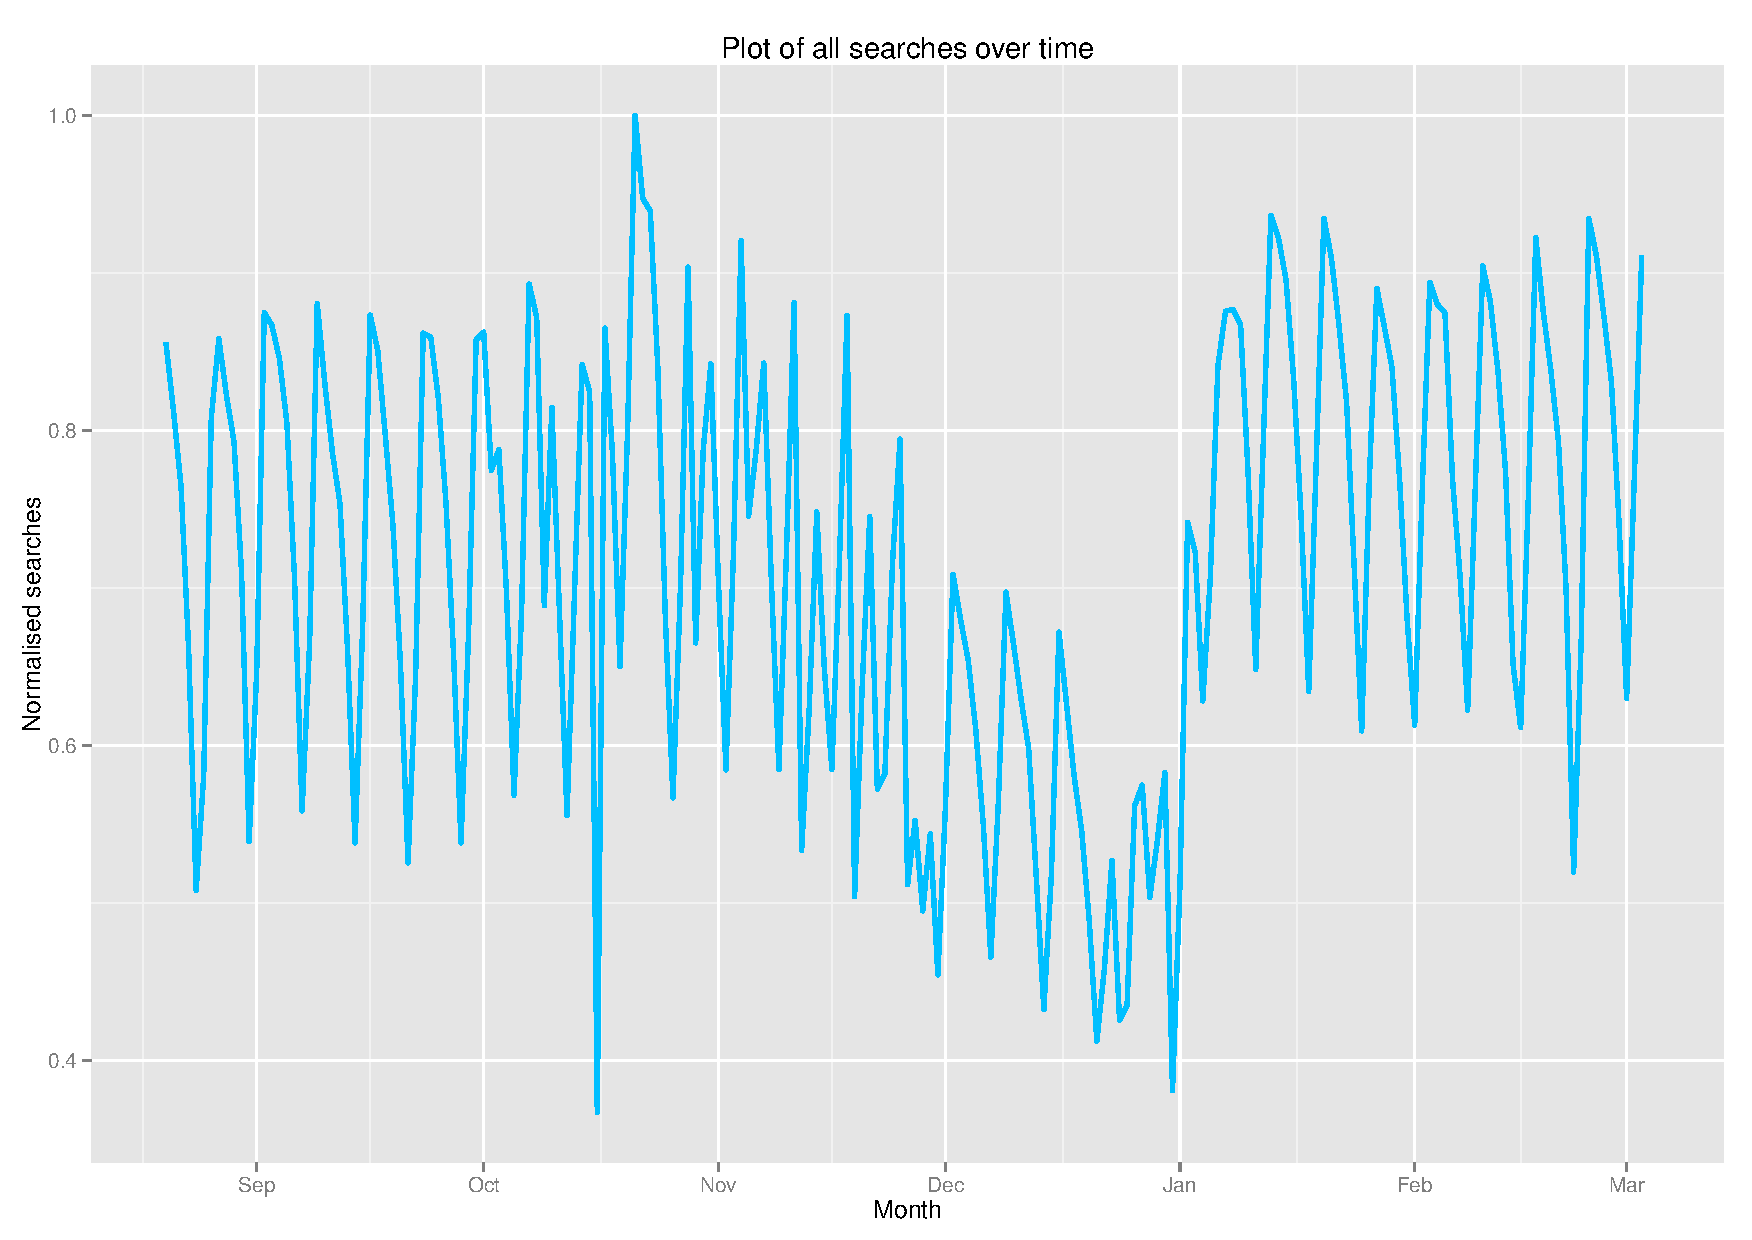
\includegraphics[scale=0.5]{overall}
\end{center}
\caption{Plot of all the searches to all the destinations. This would fall into the first group of steady constant volumes}
\label{overall-searches}
\end{figure}

%\subsection{With more features}
%
%Here
\newpage
\section{Conclusion}

The previous results have demonstrated that there is definitely a gain, even though not as great as I expected, in including exogenous factors such as Twitter in the prediction. With the first level of filtering described in chapter \ref{sec:tweettext} on page \pageref{sec:tweettext} we have achieved better prediction on slightly more than 83\% of all the destinations.  


Overall he median decrease of RMSE for TwitterDF over the Last 4 Fridays is \textbf{4\%}. With TwitterCF the median improvement is \textbf{0.6\%} across all destinations. Even though small, the gain is significant considering the events in Ukraine and Sochi and the fact that the classifier was able to take those into account shows that there is definitely some use in using exogenous factors for modelling flight search volumes. 

During the 2nd phase of the project, I will focus on retrieving only the most relevant tweets from the Twitter dataset and doing better feature extraction that will allow to remove junk features that bring the RMSE up. With that in mind, I am hopeful that I will be able to build the next version of the model that is going to perform just as well on the first group of destinations. 


\chapter{Future work}
\label{chap:future-work}


%\chapter{Timeline}

%The timeline for the next 3 months is the following:
%\begin{enumerate}
%\item Better the existing model and continue with the tests. .
%\item Add more features to the set of inputs.
%\item Work on both approaches:
%\begin{itemize}
%\item Explain spikes in searches by looking at historical tweet data
%\item Or try to predict the spikes in the first place
%\end{itemize}
%\item Final draft done by mid-March.
%\item Submit dissertation the final week of March.
%\end{enumerate}

\begin{thebibliography}{10}

\bibitem{seqcap}
	BBC, \emph{Sequoia Capital investment values Skyscanner at \$800m}, \\
	{\url{http://www.bbc.co.uk/news/uk-scotland-scotland-business-24380126}}

\bibitem{code}
	Stefan Sabev, Code for Inf Project,\\
	{\url{https://github.com/SSabev/HonsProject/}}
	
\bibitem{lasso}
	Wikipedia, \emph{Lasso (statistics)}, \\
	{\url{http://en.wikipedia.org/wiki/Lasso_(statistics)#Lasso_method}}
	
\bibitem{TwitterNewsWire}
	Twitter, \emph{Twitter as a news-wire}, \\
	{\url{https://blog.twitter.com/2008/twitter-news-wire}}

\bibitem{TwitterResearch}
	Twitter Research,
	\emph{A collection of publications using Twitter data}, \\
 	{\url{https://sites.google.com/site/twitterresearch09/twitter-papers}}

\bibitem{Miles}
	Miles Osborne, \emph{Social media papers}, \\
	{\url{http://homepages.inf.ed.ac.uk/miles/sm-papers.html}}
	
\bibitem{Petrovic2012}
	Sasa Petrovic
  	\emph{Real-time Event Detection in Massive Streams 2012} ,\\
	School of Informatics, University of Edinburgh \\
	{\url{http://homepages.inf.ed.ac.uk/s0894589/petrovic-thesis.pdf}}

\bibitem{twitstock}
	Johan Bollen, Huina Mao and Xiao-Jun Zeng, \\
	\emph{Twitter mood predicts the stock market}, \\
	{\url{http://arxiv.org/pdf/1010.3003v1.pdf}}

\bibitem{twitnfl}
	Shiladitya Sinha, Chris Dyer , Kevin Gimpel, and Noah A. Smith, \\
	\emph{Twitter mood predicts the stock market}, \\
	{\url{http://arxiv.org/pdf/1010.3003v1.pdf}}

\bibitem{twitflu}
	Michael J. Paul and Mark Dredze,  \\
	\emph{You Are What You Tweet: Analyzing Twitter for Public Health}, \\
	{\url{http://www.cs.jhu.edu/~mdredze/publications/twitter_health_icwsm_11.pdf}}

\bibitem{twitpoll}
	Brendan O'Connory,  Ramnath Balasubramanyany, Bryan R. Routledgex, Noah A. Smith, \\  
	\emph{From Tweets to Polls: Linking Text Sentiment to Public Opinion Time Series}, \\
	{\url{http://www.cs.cmu.edu/~nasmith/papers/oconnor+balasubramanyan+routledge+smith.icwsm10.pdf}}

\bibitem{dija}
	Wikipedia, \emph{Dow Jones Industrial Average}, \\
	{\url{http://en.wikipedia.org/wiki/Dow_Jones_Industrial_Average}}

\bibitem{opfind}
	OpinionFinder, \\
	{\url{http://mpqa.cs.pitt.edu/opinionfinder/}}
	
\bibitem{granger}
	Granger causality, \\
	{\url{http://en.wikipedia.org/wiki/Granger_causality}}

\bibitem{sofnn}
	Gang Leng, Girijesh Prasad, Thomas Martin McGinnity
	\emph{An on-line algorithm for creating self-organizing fuzzy neural networks} \\
	{\url{http://www.sciencedirect.com/science/article/pii/S0893608004001698}}
  
\bibitem{Hamletkdd03}
 	Etzionni, Tuchinda, Knoblock and Yates, \emph{To Buy or Not to Buy: Mining Airfare Data to Minimize Ticket Purchase Price}, 2003, \\
  	{\url{http://knight.cis.temple.edu/~yates/papers/hamlet-kdd03.pdf}}
	
\bibitem{ijcai}
	William Groves and Maria Gini, \emph{Optimal Airline Ticket Purchasing Using Automated User-Guided Feature Selection} \\
	{\url{http://ijcai.org/papers13/Papers/IJCAI13-032.pdf}}

\bibitem{samplestream}
	Twitter Sample Stream, \\
	{\url{https://dev.twitter.com/docs/api/1.1/get/statuses/sample}}
	
\bibitem{tweetobject}
	Twitter Developers Documentation, \emph{Tweets data and attributes},\\
	{\url{https://dev.twitter.com/docs/platform-objects/tweets}}

\bibitem{pandas}
	Python  \emph{Python Data Analysis Library},\\
	{\url{http://pandas.pydata.org/}}


\end{thebibliography}

\end{document}
